\documentclass[amsmath, amssymb, aps, floatfix, nofootinbib, preprintnumbers,
  showpacs, superscriptaddress, twocolumn]{revtex4-1}
\usepackage{bm}
\usepackage[cmyk]{xcolor}
\usepackage{dcolumn}
\usepackage{epsfig}
\usepackage{float}
\usepackage{graphicx}
\usepackage{multirow}
\usepackage{subfigure}
\begin{document}

\title{Studies of quantum dots}

\author{Fei Yuan}
\affiliation{National Superconducting Cyclotron Laboratory and
  Department of Physics and Astronomy,
  Michigan State University,
  East Lansing, MI 48824, USA}
\author{Sarah Reimann}
\affiliation{Department of Chemistry and Center for Theoretical and Computational Chemistry, University of Oslo, N-0316 Oslo, Norway}
\author{Scott Bogner}
\affiliation{National Superconducting Cyclotron Laboratory and
  Department of Physics and Astronomy,
  Michigan State University,
  East Lansing, MI 48824, USA}
\author{Morten Hjorth-Jensen}
\affiliation{National Superconducting Cyclotron Laboratory and
  Department of Physics and Astronomy,
  Michigan State University,
  East Lansing, MI 48824, USA}
\affiliation{Department of Physics, University of Oslo, N-0316 Oslo, Norway}


\begin{abstract}
  We present and compare several many-body methods used to study a quantum dot
  system.  We calculate the approximate ground state energy of electrons in a
  circularly symmetric potential well using a harmonic oscillator basis
  optimized via Hartree-Fock.  We further improve the ground state energy
  using in-medium similarity renormalization group (IM-SRG).  Additionally, we
  calculate the addition and removal energies using quasidegenerate
  perturbation theory (QDPT).  Our results are benchmarked against quasi-exact
  diffusion Monte Carlo results from previous works.  Possible explanations
  for the discrepancies are discussed.
\end{abstract}

\pacs{02.70.Ss, 31.15.A-, 31.15.bw, 71.15.-m, 73.21.La}
\maketitle

\section{Introduction}

Understanding the behaviour of strongly confined electrons is of fundamental
interest for solving many-body problems.  Quantum dots, e.g. electrons
confined in semiconducting heterostructures, are of particular interest since
they exhibit, due to their small size, discrete quantum levels. Under these
conditions, typical quantum phenomena like tunnelling, entanglement and
magnetization can all be observed \cite{reimann2002,engel1993}.  Since quantum
dots are manufactured and designed artificially at the laboratory, their
quantum levels can be tuned to one's needs by changing for instance the
external field, or the size and shape of the system. As a consequence, quantum
dots provide a high level of control for the dynamics and correlation of the
electrons, which makes them perfectly suited to study quantum effects in
practice.  Since their ground state shows similar shell structures and magic
numbers as seen for atoms and nuclei \cite{tarucha1996}, these systems give
the opportunity to study electronic systems without the presence of a nucleus
affecting the electrons.  Apart from their relevance for theoretical research
in quantum physics, quantum dots offer a wide variety of applications: In
particular, their electrical and optical properties make them attractive for
the use in laser technology \cite{strauf2010,5075760} and solar cells
\cite{jenks:013111,doi:10.1021/cr900289f}, but they are also used in quantum
computers \cite{PhysRevA.57.120} and medical imaging \cite{Ben-Ari02042003}.

In order to properly understand the properties of quantum dots and make
theoretical predictions to their behaviour in various applications, it is
necessary to study features like ground state energy and correlation
effects. Since apart from quantum dots consisting of only two electrons or
with specific values of the external field, no analytical solutions exist
\cite{PhysRevA.48.3561}, the development of appropriate few- and many-body
methods is required.

Several \textit{ab initio} methods have been applied to these systems, in
particular variational and diffusion Monte Carlo \cite{PhysRevB.68.035304,%
  PhysRevB.62.8120,PhysRevB.84.115302,PhysRevB.54.4780}, large-scale
diagonalization \cite{JJAP.36.3924,PhysRevB.56.6428,Kvaalcode,rontani:124102}
and Coupled Cluster theory \cite{PhysRevB.67.045320,heidari:114708,%
  PhysRevB.84.115302}.

Additionally to those approaches, another very promising first-principle
method has recently evolved. This is the Similarity Renormalization Group
(SRG) method, which drives the Hamiltonian to a band- or block-diagonal form
using a continuous series of unitary transformations.  Especially in nuclear
theory, it has successfully been applied to study systems with different
underlying potentials, and it has been used to analyse their binding energy
and other observables \cite{ScottSRG,PhysRevC.75.061001,SRGThreeDim}. Apart
from the free-space approach, where the Hamiltonian is set up with respect to
the zero vacuum state, in recent times another interesting alternative has
been worked out: Making use of the technique of normal-ordering, the SRG
evolution is performed in medium, where 3, \ldots, $A$-body operators can be
approximated using only two-body machinery. This in-medium SRG (IM-SRG) allows
considerable simplifications to the problem and makes numerical calculations
much more efficient \cite{IMSRG}.

 This article is organized as follows: Section \ref{sec:formalism}
 introduces first (\ref{subsec:modelHamiltonian}) the Hamiltonian we
 use to model circular quantum dots, and gives afterwards an overview
 over the SRG (\ref{subsec:SRG}) and DMC (\ref{subsec:DMC})
 formalism. Our results are presented in Section \ref{sec:results}. We
 point out the differences arising from the use of two different
 generators, Wegner's and White's one, and give an overview over the
 ground state energies up to 42 particles. In particular, we compare
 the results obtained with five different \textit{ab initio} methods:
 IM-SRG(2), DMC, Hartree-Fock, Full Configuration Interaction and
 Coupled Cluster. Section \ref{sec:conclusions} concludes our work and
 gives perspectives for future work.

The harmonic oscillator (HO) is ubiquitous in quantum physics. It is
the basis for extremely diverse many-body calculations in nuclear
physics,\cite{HjorthJensen1995} quantum chemistry,\cite{Helgaker2002}
and quantum dot calculations in solid state physics.\cite{Reimann2002}
In these calculations, one typically seeks a few of the lowest
eigenenergies $E_k$ of the system Hamiltonian $H$, and their
corresponding eigenvectors $\psi_k$, viz,
\[ H\psi_k = E_k\psi_k, \quad k = 1,\cdots,k_\text{max}. \] In all
cases, the many-body wave function is expanded in a basis of
eigenfunctions of the HO, and then necessarily truncated to give an
approximation. In fact, the so-called curse of dimensionality implies
that the number of degrees of freedom per particle available is
severely limited. It is clear, that an understanding of the properties
of such expansions, giving \emph{a priori} error estimates on
many-body calculations, is very important. Unfortunately, this is a
neglected topic in the physics literature. In this article, we give a
thorough mathematical and numerical analysis and give practical
convergence estimates of HO basis expansions. It generalizes and
refines the findings of a recent study of one-dimensional systems.\cite{Kvaal2007}


The HO eigenfunctions are popular for several reasons. Many quantum
systems, such as the quantum dot model considered here, are perturbed
harmonic oscillators \emph{per se}, so that the true eigenstates
should be perturbations of the HO states. Moreover, the HO has many
beautiful properties, such as separability, invariance under
orthogonal coordinate changes, and easily computed eigenfunctions, so
that computing matrix elements of relevant operators becomes
relatively simple. The HO eigenfunctions are defined on the
\emph{whole} of $\mathbb{R}^d$ in which the particles live, so that
truncation of the domain is unnecessary. Indeed, this is one of the
main problems with methods such as finite difference or finite element
methods.\cite{RamMohan2002}


\section{Formalism}
\label{sec:formalism}

\subsection{The model Hamiltonian}
\label{subsec:modelHamiltonian}

We model the quantum dot as a collection of $N$ electrons trapped in an
external harmonic-oscillator potential.\footnote{In this paper, we use atomic
  units where $\hbar$, $m$, $e$, and $4 \pi \epsilon$ are unity, with
  $\epsilon$ denoting the permittivity and $m$ denoting the mass, which may be
  an effective mass.  In vacuum where $m = m_{\text e}$ and
  $\epsilon = \epsilon_0$, energy would be measured in units of hartrees
  $E_{\text h} \equiv m_{\text e} (\alpha c)^2$.  More generally, the units of
  energy are $m_{\text r \vphantom h}^{} E_{\text h}^{} /
  \epsilon_{\text r \vphantom h}^2$ where
  $\epsilon_{\text r} \equiv \epsilon / \epsilon_0$ and
  $m_{\text r} \equiv m / m_{\text e}$.}  Each electron possesses kinetic
energy $t(\bm p) \equiv \bm p^2 / 2$ and experiences an external potential
\begin{align*}
  u(\bm r) \equiv \frac{1}{2} \omega^2 \bm r^2
\end{align*}
where $\omega$ is the angular frequency of the oscillator, $\bm r$ is the
2-dimensional coordinate of an electron, and $\bm p$ is its momentum.  Each
pair of electrons experience a Coulomb repulsion
\begin{align*}
  v(\bm r, \bm r') \equiv \frac{1}{|\bm r - \bm r'|}
\end{align*}
where $\bm r$ and $\bm r'$ are coordinates of a pair of electrons.  Thus, the
full many-body problem is described by the nonrelativistic Hamiltonian
\begin{align*}
  \hat H \equiv \sum_{p} \bigl(
  t(\hat{\bm p}_p) + u(\hat{\bm r}_p)
  \bigr) + \sum_{\{p, q\}} v(\hat{\bm r}_p, \hat{\bm r}_q)
\end{align*}
where $\hat{\bm p}_p$ is the momentum operator and $\hat{\bm r}_p$ is the
position operator for a particle labeled by $p$.  The first summation is
performed over every particle $p$, while the the second summation is performed
over every unordered pair of particles $\{ p, q \}$ (with $p \ne q$).

The full problem is not a trivial one.  We shall first consider a much simpler
problem: a noninteracting Hamiltonian $\hat H^{\text o}$ in which the Coulomb
interaction $v$ is removed:
\begin{align*}
  \hat H^{\text o} \equiv \sum_{p} \bigl(
  t(\hat{\bm p}_p) + u(\hat{\bm r}_p)
  \bigr)
\end{align*}
In this case, the many-body Hamiltonian reduces to $N$ independent
single-particle Hamiltonians, each of the form:
\begin{align*}
  \hat h^{\text o} \equiv
  \frac{\hat{\bm p}^2 + \omega^2 \hat{\bm x}^2}{2}
\end{align*}
This is a 2-dimensional harmonic oscillator problem for a single particle,
whose solutions are well known.  There are, however, various ways to construct
the set of eigenfunctions: we shall use the Fock-Darwin states that conserve
angular momentum about the axis perpendicular to the plane.  The
eigenfunctions have the following analytic form in polar
coordinates:\citep[Appx.\ A]{lohne2010coupled}
\begin{gather*}
  \phi^{\text{fd}}_{n, m_\ell}(r, \varphi)
  \equiv \sqrt\omega
  \phi^{\text{fdr}}_{n, |m_\ell|}(\sqrt \omega r)
  \phi^{\text{fda}}_{m_\ell}(\varphi)
\end{gather*}
where
\begin{align*}
  \phi^{\text{fdr}}_{n, \mu}(\rho) &\equiv
  \sqrt{\frac{2 \cdot n!}{(n + \mu)!}}
  {\mathrm e}^{- \rho^2 / 2} \rho^\mu L_n^{(\mu)}(\rho^2) \\
  \phi^{\text{fda}}_{m_\ell}(\varphi) &\equiv
  \frac{1}{\sqrt{2 \pi}} {\mathrm e}^{i m_\ell \varphi}
\end{align*}
and $L_n^{(\mu)}$ denotes the generalized Laguerre polynomial of degree $n$
with parameter $\mu$.  The states are labelled by two quantum numbers: the
principal quantum number $n \in \{0, 1, \ldots\}$ and the angular momentum
projection $m_\ell \in \mathbb Z$.

Additionally, since electrons are spin-$1/2$ fermions, they can occupy either
of the two spin states $\chi_{+\frac12}$ or $\chi_{-\frac12}$.  Thus, the
single-particle basis states can be constructed as
\begin{align} \label{eq:singleparticlestate}
  \phi_{n, m_\ell, m_{\text s}}(r, \varphi) \equiv
  \phi^{\text{fd}}_{n, m_\ell}(r, \varphi) \chi_{m_{\text s}}
\end{align}
with the spin projection $m_{\text s} \in \bigl\{-\frac12, +\frac12\bigr\}$.

\begin{figure}
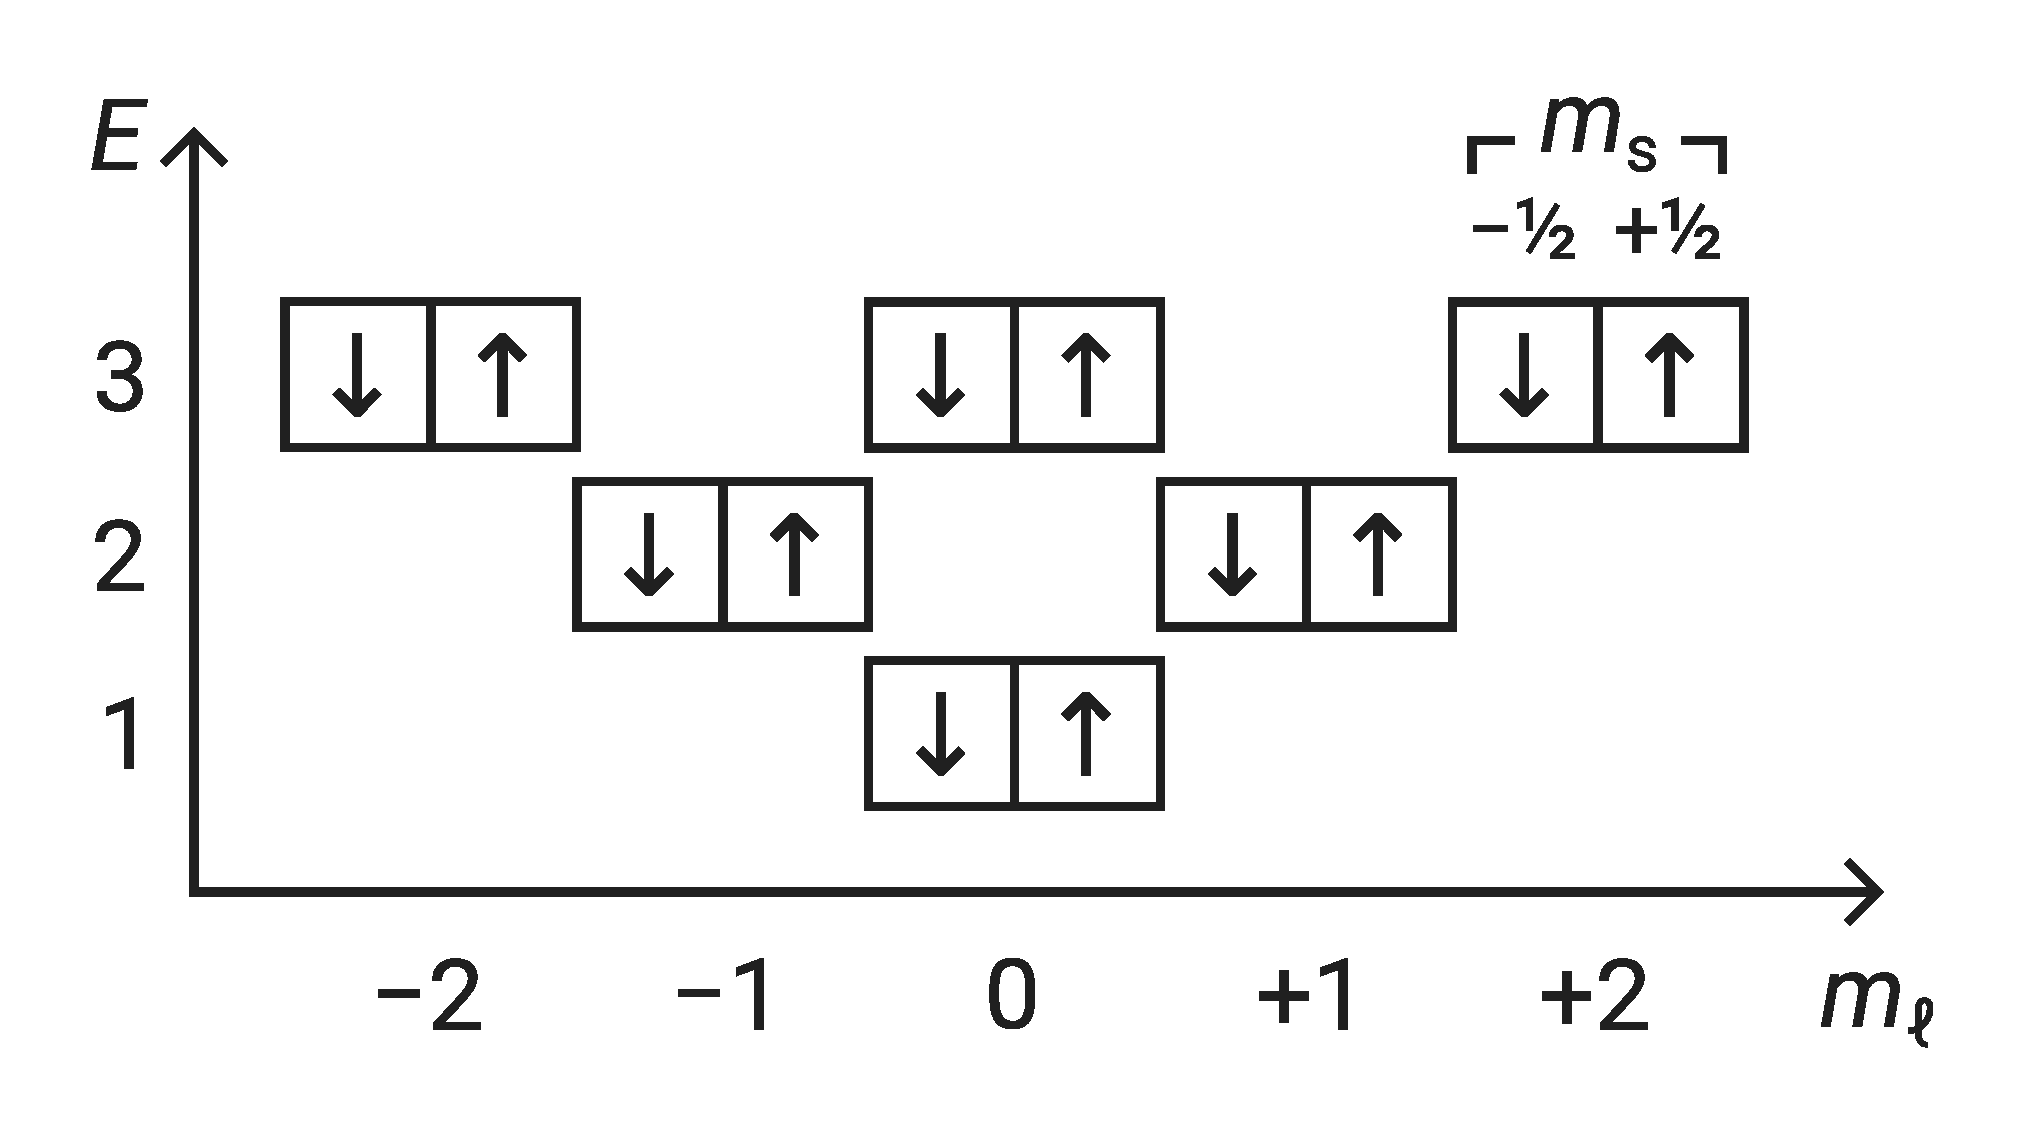
\includegraphics[width=.48\textwidth]{fig-shell-structure}
\caption{Structure of the single-particle states in a noninteracting harmonic
  oscillator.}
\label{fig:shell-structure}
\end{figure}
The eigenvalues of the single-particle Hamiltonian $\hat h^{\text o}$ are
given by
\begin{align*}
  \varepsilon_{n, m_\ell, m_{\text s}} \equiv (2 n + |m_\ell| + 1) \omega
\end{align*}
Note that they are degenerate with respect to the spin projection
$m_{\text s}$ since our Hamiltonian $\hat h^{\text o}$ does not distinguish
between them.  From this equation, we can see that the single-particle basis
states form a shell structure as shown in Figure \ref{fig:shell-structure}.
Every state within a given shell is degenerate and states within a given shell
satisfy $2 n + |m_\ell| = k$ for some nonnegative integer $k$, which we call
the \textit{shell index}.  The shells are equidistant from each other, with a
spacing equal to the frequency $\omega$.

The many-body Hamiltonian $\hat H^{\text o}$ is the sum of the single-particle
Hamiltonians $\hat h^{\text o}_p$ over all particles $p$, where $p$ may now be
treated as a tuple of all three single-particle quantum numbers:
$(n, m_\ell, m_{\text s})$.  From the states $\phi$ in
\eqref{eq:singleparticlestate} we can construct the eigenstates of the
many-body Hamiltonian $\hat H^{\text o}$ in the form of Slater determinants
that automatically satisfy the Pauli exclusion principle:
\begin{align*}
  \Phi_{p_1, \ldots, p_N}(\bm r_1, \ldots, \bm r_N) \equiv
  \frac{1}{\sqrt{N}} \left|
  \begin{matrix}
    \phi_{p_1}(\bm r_1) & \cdots & \phi_{p_N}(\bm r_1) \\
    \vdots & \ddots & \vdots \\
    \phi_{p_1}(\bm r_N) & \cdots & \phi_{p_N}(\bm r_N) \\
  \end{matrix}
  \right|
\end{align*}
The energy of these states is given by the sum of the single-particle
energies:
\begin{align*}
  E^{\text o}_{p_1, \ldots, p_N} \equiv
  \varepsilon_{p_1} + \cdots + \varepsilon_{p_N}
\end{align*}
For ground states, we may have degeneracies due to the shell structure of the
single-particle basis.  However, if $N = k_{\text f} (k_{\text f} + 1)$ for
some nonnegative integer $k_{\text f}$, there are just enough particles to
form a closed-shell system.  In this case, there is a unique, well-isolated
ground state.  The values of $N$ for which this occurs are typically referred
to as \textit{magic numbers} and we call $k_{\text f}$ the \textit{number of
  filled shells}.  This completes the solution of the noninteracting problem.

The difficulty in solving the full Hamiltonian $\hat H$ stems from the fact
that the exact solution cannot be expressed in terms of a single Slater
determinant due to the presence of interactions.  Hence, it is not possible to
reduce the problem to that of a single particle as we had done previously.

However, if we assume that the interaction alters the behavior of the system
only mildly, we can use the Slater determinants of the noninteracting system
as an initial guess for the solution, and then apply iterative methods to
improve the accuracy of the solution.

Since Slater determinants are rather cumbersome to write out in full, we shall
instead work in the more convenient formalism of second quantization:
\begin{align*}
  |\Phi_{p_1, \ldots, p_N}\rangle =
  \hat a_{p_1}^\dagger \cdots \hat a_{p_N}^\dagger |\varnothing\rangle
\end{align*}
Here, $\hat a_p^\dagger$ is the creation operator for the single-particle
state $p$ and $|\varnothing\rangle$ is the (true) vacuum state that is devoid
of particles.  Analogously, $\hat a_p$ is the annihilation operator for the
state $p$.

Operators can be rewritten in this formalism as well.  The one-body kinetic
energy operator, defined by
\begin{align*}
  \hat T \equiv \sum_p \hat t(\hat{\bm p}_p)
\end{align*}
can be rewritten in second quantization as
\begin{align*}
  \hat T = \sum_{p, q} T_{p, q}^{} \hat a_p^\dagger \hat a_q^{}
\end{align*}
where the operator matrix element
$T_{p, q} \equiv \langle \Phi_p | \hat T | \Phi_q \rangle$.  This can likewise
be extended for both $\hat U$ and $\hat V$,
\begin{align*}
  \hat U &= \sum_{p, q} U_{p, q}^{} \hat a_p^\dagger \hat a_q^{} \\
  \hat V &= \frac{1}{4} \sum_{p, q, r, s} V_{p, q, r, s}^{}
  \hat a_p^\dagger \hat a_q^\dagger \hat a_s^{} \hat a_r^{}
\end{align*}
where $U_{p, q} \equiv \langle \Phi_p | \hat U | \Phi_q \rangle$ and
$V_{p, q, r, s} \equiv \langle \Phi_{p, q} | \hat V | \Phi_{r, s} \rangle$.
Note that due to the antisymmetry present in the Slater determinants, we have
the property that exchanging either $p$ with $q$ or $r$ with $s$ causes
$V_{p, q, r, s}$ to reverse in sign.

\subsection{Hartree-Fock method}
\label{subsec:HartreeFockmethod}

The first correction that we will apply to our solution is that of the
Hartree-Fock method.  Using the variational principle, we compute an
approximate ground state $\Psi^{\text{hf}}$ by minimizing the energy
\begin{align*}
  E^{\text{hf}} \equiv \langle \Psi^{\text{hf}} | \hat H | \Psi^{\text{hf}} \rangle
\end{align*}
with respect to $\Psi^{\text{hf}}$, subject to the restriction that
$\Psi^{\text{hf}}$ is a single Slater determinant constructed from a set of
$N$ orthonormal single-particle states.  We denote each state $\psi_u$, where
$u$ is its label.

To make this computationally feasible, we further assume that the unknown
states $\psi$ are built from a linear combination of known functions,
drawn from a finite set.  This reduces the problem from an abstract
mathematical one to a numerical linear algebra problem, with the caveat that
this set of known functions must be chosen carefully.

Assuming the interaction is not too strong, we can use the single-particle
states $\phi$ of our noninteracting Hamiltonian as a basis for the unknown
states $\psi$.  The two sets of states are then related by a linear
transformation $\bm C$:
\begin{align*}
  \psi_u \equiv \sum_p \phi_p C_{p, u}
\end{align*}
To ensure the orthonormality of the states, we expand the set of unknown
states $\psi$ to have as many elements as the set of $\phi$ and require the
\textit{coefficient matrix} $\bm C$ to be unitary.  While these conditions
are more strict than necessary, they greatly simplify the calculations and the
additional states are essential inputs for methods beyond Hartree-Fock.  The
set of states $\psi$ now consists of $N$ \textit{occupied} states that
participate in the Slater determinant $\Psi^{\text{hf}}$ and the remaining
\textit{unoccupied} states that do not.

Since the coefficient matrix uniquely determines the unknown states, the
variational problem has been reduced to that of solving of the coefficients
$\bm C$ that minimize the energy $E$, which is given by
\begin{align*}
  E^{\text{hf}} = \sum_{\underline u} C_{p, u}^* H_{p, q}^{\text o} C_{q, u}^{}
  + \sum_{\underline u, \underline v}
  C_{p, u}^* C_{q, u}^* V_{p, q, r, s}^{} C_{r, u}^{} C_{s, u}^{}
\end{align*}
where the underlined indices indicate that the summation is over occupied
states only.

Using the method of Lagrange multiplers, the minimization problem can be
reduced to the solving of a nonlinear equation -- the \textit{Hartree-Fock
  equation}:
\begin{align} \label{eq:hartreefock}
  \bm f \bm C = \bm C \bm \epsilon
\end{align}
where the \textit{Fock matrix} $\bm f$ is defined as
\begin{align} \label{eq:fock}
  f_{p, r} \equiv H_{p, r}^{\text o} + \sum_{\underline u q s}
  C_{q, u}^* V_{p, q, r, s}^{} C_{s, u}^{}
\end{align}
and $\bm \epsilon$ is a vector of Lagrange multipliers with each
element $\epsilon_u$ associated with a particular state $u$.  While the Fock
matrix $\bm f$ may appear to be an artificial Hamiltonian derived purely
from the minimization problem, it can be generalized as an operator whose
relevance extends beyond Hartree-Fock.

The Hartree-Fock equation can be solved by an iterative technique: a solution
$\bm C$ can be fed into \eqref{eq:fock} and new solution can then obtained
by solving the eigenvalue problem in \eqref{eq:hartreefock} using the Fock
matrix obtained.  For the initial guess, we use the ground state of our
noninteracting Hamiltonian, thus $\bm C$ is initially the identity matrix.

Since Hartree-Fock method restricts the ground state to a Slater determinant
of single-particle states, it cannot provide an exact solution to a problem
where correlation is present, even if the basis $\phi$ is infinite.  The
energy difference between the best Hartree-Fock energy and the exact ground
state energy is thus by definition known as the \textit{correlation energy}.
There are various methods of recovering (at least parts of) this missing
energy.  The focus of this paper shall be on the IM-SRG method.

\subsection{The IM-SRG method}
\label{subsec:imsrgmethod}

In the similarity renormalization group (SRG) method, one performs a
continuous sequence of unitary transformations on a Hamiltonian operator
$\hat H$ to evolve it into a more ``amenable'' form -- which generally implies
decoupling a small model space of interest from its complement.  The sequence
is parameterized by a continuous variable $s$ known as the \textit{flow
  parameter}, which by convention we define to be $0$ at the beginning of the
sequence.  Upon reaching $s$, the transformed Hamiltonian is given by
\begin{align*}
  \tilde H(s) \equiv \hat U(s) \hat H \hat U(s)
\end{align*}
where $U(s)$ describes the product of all such transformations since $s = 0$.
At every step $s'$, the differential unitary transformation is described by
the exponential of an antihermitian operator $\eta(s)$, known as the
\textit{generator} of the transformation.  When ``integrated'' as a product,
the full transformation $\hat U(s)$ is recovered:\footnote{Alternatively, this
  can also be reinterpreted as an $s'$-ordered integral.  See \cite[\S
  6.1]{reimann2013quantum}.}
\begin{align*}
  \hat U(s) = \lim_{\Delta s' \to 0} \prod_{s' = 0}^{s' = s}
  \mathrm e^{\hat \eta(s') \Delta s'}
\end{align*}
The evolution of the Hamiltonian itself is governed by a differential
equation, commonly referred to as the flow equation:
\begin{gather} \label{eq:imsrgode}
  \frac{d}{d s} \tilde H(s) = [\hat \eta(s), \tilde H(s)]
\end{gather}
which allows $\tilde H(s)$ to be evaluated without explicitly constructing the
full transformation $\hat U(s)$.

 Introducing a flow parameter $s$, there exits a unitary
 transformation $U_s$, such that
\begin{equation}
 \hat{H}_s = U_s^\dagger \hat{H} U_s \equiv \Hd_s + \Ho_s,
\end{equation}
with the relations $U_{s=0} = \mathbf{1}$, and $\hat{H}_{s= 0} =
\hat{H}$.  The transformation $U_s$ is parametrized as
\[
U_s = T_s \exp \left(\int_0^s \! ds'\hat{\eta}_{s'} \right),
\]
where the anti-hermitian operator $\hat{\eta}_s$ serves as generator
of the transformation. With $T_s$ we denote $s$-ordering, which is
defined equivalently to usual time-ordering.  Taking the derivative of
$\hat{H}_s$ with respect to $s$ gives
\begin{equation}
 \frac{d \hat{H}_s}{ds} = \frac{d U_s}{ds}\hat{H} U_s^\dagger + U_s
 \hat{H} \frac{d U_s^\dagger}{ds}.
\label{eq:flow_long}
\end{equation}
Utilizing that for our particular form of $U_s$, we have that \be
\hat{\eta}_s = \frac{d U_s}{ds} U_s^\dagger = - U_s \frac{d
  U_s^\dagger}{ds} = -\hat{\eta}_s,
\label{eq:eta}
\ee we obtain that \be \frac{d \hat{H}_s}{ds} = \hat{\eta}_s \hat{H}_s
- \hat{H}_s \hat{\eta}_s = \left[\hat{\eta}_s, \hat{H}_s \right].
\label{eq:flowEquations}
\ee This is the key expression of the SRG method, describing the flow
of the Hamiltonian.  The specific unitary transformation is determined
by the choice of $\hat{\eta}_s$.  Through different choices of
$\hat{\eta}_s$, the SRG evolution can be adapted to the features of a
particular problem.\\

\paragraph*{In-medium SRG}

One possibility to solve the flow equations is to choose a basis with
respect to the physical vacuum state, set up the Hamiltonian matrix in
this basis and solve Eq.~(\ref{eq:flowEquations}) as a set of coupled
first-order differential equations. However, since the size of the
problem grows enormously with the number of particles and the size of
the model space, the applicability of this free-space SRG method is
restricted to comparatively small systems.

Instead of performing SRG in free space, the evolution can be done at
finite density, i.e.~directly in the A-body system
\cite{kehrein2006flow}. This approach has recently been applied very
successfully in nuclear physics \cite{IMSRG,PhysRevLett.106.222502}
and is called in-medium SRG (IM-SRG). The method allows the evolution
of $3,...,A$-body operators using only two-body machinery, with the
simplifications arising from the use of normal-ordering with respect
to a reference state.

In our case, we assume that the problem can be modelled by a
Hamiltonian containing maximally two-body interactions. In
second-quantized form, this one is given by
\begin{align}
\hat{H} & = \sum\limits_{pq}\left\langle p \right| \hat{h}^{(0)}
\left| q \right\rangle a_p\da a_q + \frac{1}{4}\sum\limits_{pqrs}\lla
pq || r s \rra a_p\da a_q\da a_s a_r,
\label{eq:ourHamiltonian}
\end{align} 
where the operator $\hat{h}^{(0)}$ denotes the single-particle
Hamiltonian, and the elements $\langle pq||rs\rangle$ are the
anti-symmetrized two-body matrix elements.  Normal-ordering with
respect to a reference state $|\Phi_0\rangle$ yields
\begin{align*}
\hat{H} &= E_0 + \sum\limits_{pq}f_{pq}\llb a_p\da a_q\rrb +
\frac{1}{4}\sum\limits_{pqrs}v_{pqrs} \llb a_p\da a_q\da a_s a_r \rrb,
\end{align*}
with Fock matrix elements
\[
f_{pq} = \lla p \right|\hat{h}^{(0)}\left| q \rra + \sum\limits_{i}
\lla pi || qi\rra,
\]
and where $v_{pqrs} = \lla pq || r s \rra$ are the amplitudes of the
two-body operator.  Here and in the following, indices $i,j,k,...$
denote hole states below the Fermi level, indices $a,b,c,...$
particles states above the Fermi level, and indices $ p,q,r,...$ can
be used for both particle and hole states. As reference state
$|\Phi_0\rangle$ we choose the ground state of the non-interacting
system, where all single-particle orbitals below the Fermi level are
occupied.

Integrating the flow equations~(\ref{eq:flowEquations}), we face one
of the major challenges of the SRG method, namely the generation of
higher and higher order interaction terms during the flow. With each
evaluation of the commutator, the Hamiltonian gains terms of higher
order, and these induced contributions will in subsequent integration
steps contribute to terms of lower order. In principle, this continues
to infinity.\\ To make the method computationally possible, we have to
close the IM-SRG flow equations, suggesting that we are forced to
truncate the equations to a certain order. We choose to truncate both
$\hat{H}_s$ and $\hat{\eta}_s$ at the two-body level, an approach
which is referred to as IM-SRG(2).  This normal-ordered two-body
approximation seems to be sufficient in many cases and has yielded
excellent results for several nuclei
\cite{PhysRevLett.106.222502,PhysRevLett.109.052501,IMSRG}.\\ The
commutator in the flow equations (\ref{eq:flowEquations}) guarantees
that the IM-SRG wave function $U_s^\dagger|\Phi\rangle$ can be
expanded in terms of linked diagrams only
\cite{shavitt2009many,ISI:A1981MN73700014}, which suggests that IM-SRG
is size-extensive. Regarding the quality of the SRG results, it means
that the error introduced by truncating the many-body expansions
scales linearly with the number of particles~$N$.\\ With this
truncation, the generator $\hat{\eta}$ can be written as
\[
\hat{\eta} = \sum_{pq} \eta_{pq}^{(1)} \llb a_p\da a_q\rrb +
\frac{1}{4}\sum\limits_{pqrs}\eta_{pqrs}^{(2)} \llb a_p\da a_q\da a_s
a_r \rrb,
\]
where $\eta_{pq}^{(1)}$ and $ \eta_{pqrs}^{(2)}$ are the one- and
two-body elements, respectively. Making use of the permutation
operator $ \hat{P}_{pq}f(p,q) = f(q,p)$, the IM-SRG(2) flow equations
are given by
\begin{widetext}
\begin{align}
\frac{d E_0}{ds} &= \sum_{ia}\left( \eta_{ia}^{(1)}f_{ai} -
\eta_{ai}^{(1)}f_{ia}\right) +
\frac{1}{2}\sum_{ijab}\eta_{ijab}^{(2)}v_{abij},
\label{eq:flow1}\\
\frac{d f_{pq}}{ds}&= \sum_r \lb \eta_{pr}^{(1)}f_{rq} +
\eta_{qr}^{(1)}f_{rp}\right) + \sum_{ia}\lb 1-\hat{P}_{ia}\rb \lb
\eta_{ia}^{(1)}v_{apiq} - f_{ia}\eta_{apiq}^{(2)} \rb \notag \\ &
+\frac{1}{2} \sum_{aij} \lb 1+\hat{P}_{pq}\rb
\eta_{apij}^{(2)}v_{ijaq} + \frac{1}{2}\sum_{abi}\lb 1+\hat{P}_{pq}\rb
\eta_{ipab}^{(2)}v_{abiq},
\label{eq:flow2}
\end{align}
\begin{align}
\frac{d v_{pqrs}}{ds} &= \sum_t \lb 1-\hat{P}_{pq} \rb \lb
\eta_{pt}^{(1)}v_{tqrs}-f_{pt}\eta_{tqrs}^{(2)}\rb -\sum_t \lb
1-\hat{P}_{rs} \rb \lb \eta_{tr}^{(1)} v_{pqts} - f_{tr}
\eta_{pqts}^{(2)}\rb \notag \\ & +\frac{1}{2}\sum_{ab}
\lb\eta_{pqab}^{(2)} v_{abrs} - v_{pqab}\eta_{abrs}^{(2)}\rb -
\frac{1}{2}\sum_{ij} \lb\eta_{pqij}^{(2)} v_{ijrs} -
v_{pqij}\eta_{ijrs}^{(2)}\rb \notag \\ & -\sum_{ia} \lb 1-
\hat{P}_{ia} \rb \lb 1-\hat{P}_{pq}\rb \lb 1-\hat{P}_{rs} \rb
\eta_{aqis}^{(2)}v_{ipar}.
\label{eq:flow3}
\end{align}
\end{widetext}
Note that for brevity, we skip all $s$-dependence in the equations.

\subsubsection*{Choice of generator}
To determine the specific unitary transformation, one needs to specify
the generator~$\hat{\eta}$. Through different choices, the SRG flow
can be adapted to the features of a particular problem.\\


\paragraph*{Wegner's canonical generator}
The original choice, suggested by Wegner \cite{PhysRepWegner0}, reads
\be \hat{\eta} = \left[ \Hd, \Ho \right] = \left[ \Hd, \hat{H}
  \right].
\label{eq:etaWegner}
\ee As commutator between two Hermitian operators, $\hat{\eta}$
fulfils the criterion of antihermiticity and can be shown to suppress
the off-diagonal matrix elements \cite{kehrein2006flow}. In general,
matrix elements far off the diagonal, where the Hamiltonian connects
states with large energy differences, are suppressed much faster than
elements closer to the diagonal. \\ Evaluating the commutator, we get
for the one- and two-body elements
\begin{align*}
\eta_{pq}^{(1)} = & \sum_{r}\lb f_{pr}^d f_{rq} - f_{pr} f_{rq}^d \rb
+ f_{pq} v_{qppq}^d \lb n_q - n_p \rb \\ \eta_{pqrs}^{(2)} = & -
\sum_t \left\lbrace \lb 1-\hat{P}_{pq} \rb f_{pt} v_{tqrs}^d - \lb 1 -
\hat{P}_{rs} \rb f_{tr} v_{pqts}^d \right\rbrace \notag \\ & + \sum_t
\left\llb \lb 1 - \hat{P}_{pq} \rb f_{pt}^d v_{tqrs} - \lb 1 -
\hat{P}_{rs} \rb f_{tr}^d v_{pqts} \right\rrb \notag \\ & +
\frac{1}{2} \sum_{tu} (1 - n_t - n_u) \lb v_{pqtu}^d v_{turs} -
v_{pqtu} v_{turs}^d \rb \notag \\ & + \sum_{tu} \lb n_t - n_u \rb \lb
1 - \hat{P}_{pq} \rb \lb 1 - \hat{P}_{rs} \rb v_{tpur}^d v_{uqts},
\end{align*}
where we use the standard notation
\[
n_p = \begin{cases} 1, & \mbox{if } p< \epsilon_F \quad(p\;\mbox{is
    hole state})\\ 0, &\mbox{if } p> \epsilon_F \quad(p\;\mbox{is
    particle state})\\
\end{cases}.
\]

\paragraph*{White's generator}
Apart from this canonical generator, there exist several other ones in
literature. One of them is White's choice
\cite{White:cond-mat0201346}, which makes numerical approaches much
more efficient.  The problem with Wegner's generator are the widely
varying decaying speeds of the elements, removing first terms with
large energy differences and then subsequently those ones with smaller
energy separations.  That way the flow equations become a stiff set of
coupled differential equations, which often gets numerically
unstable.\\ White takes an alternative approach, which is especially
suited for problems where one is interested in the ground state of a
system. Instead of driving all off-diagonal elements of the
Hamiltonian to zero, he focuses solely on those ones that are
connected to the reference state $|\Phi_0\rangle$, aiming to decouple
the reference state from the remaining Hamiltonian. With a suitable
transformation, the elements get similar decaying speeds, which solves
the problem of stiffness of the flow equations.  The generator is
explicitly constructed the following way
\cite{PhysRevLett.106.222502,White:cond-mat0201346}
\begin{align}
\hat{\eta} &= \sum_{ai} \frac{f_{ai}}{f_a-f_i-v_{aiai}}\lbrace a_a\da a_i\rbrace -\text{hc} \notag \\ & + \sum_{abij}
\frac{v_{abij}}{f_a+f_b-f_i-f_j+A_{abij}}\lbrace a_a\da a_b\da a_j
a_i\rbrace - \text{hc},
\label{eq:WhiteFull}
\end{align}
with $f_p \equiv f_{pp}$, 'hc' denoting the Hermitian conjugate, and
\[
A_{abij} = v_{abab} + v_{ijij} - v_{aiai} - v_{ajaj} - v_{bibi} -
v_{bjbj}.
\label{eq:White7}
\]
Compared to Wegner's canonical generator, where the final flow
equations involve third order powers of the $f$- and $v$-elements,
these elements contribute only linearly with White's generator, which
results in much better numerical properties.




We may attempt follow the same technique as for Hartree-Fock and reduce the
operator problem into a linear algebra problem by evaluating the operator
using a single-particle basis.  However, since a commutator between two-body
operators can result in a three-body operator, it follows that as $s$
increases, the evolved Hamiltonian $\tilde H(s)$ can gain terms that couple
more and more particles.  It is not practical to keep all such terms,
especially since higher-body operators are much more computationally
expensive.

In-medium SRG follows the same procedure as with ordinary SRG, but the
calculations are performed relative to some reference state rather than the
vacuum state.  This is advantageous for systems with many-particles as the
effect of truncation is not quite as drastic as it would be in SRG
[[true/false?]].

[[need some more content before diving straight into the algebra]]

Normal-ordering is a syntactic operation that reorders a product of operators
so as to eliminate all but the highest-body interaction.  The operation is
must be defined against a fixed many-body state, such as the vacuum state.  We
denote normal ordering using $\mathopen: \ldots \mathclose:$, with with the
state given by context.

\textit{Normal-ordering with respect to the vacuum state} is performed by
rearranging the operator product such that every $\hat a^\dagger$ appear
before $\hat a$, with the caveat that the parity of the permutation must also
be applied to the sign of the result.

For many-body problems involving large number of particles, the vacuum state
is not very convenient as it requires the application of many creation
operators to reach the states of interest.  Therefore, it is preferable to
utilize some reference state $\Phi$ (a Slater determinant) so that any other
state can be readily expressed as some excitation from this state.

Given a reference state $\Phi$, we may define a set of \textit{quasiparticle
  creation and annihilation operators} $\hat b^\dagger$ and $\hat b$ that obey
the same commutation relations as the $\hat a$ operators.  The two sets of
operators are related by:
\begin{align*}
  \hat b_p^\dagger \equiv \begin{cases}
    \hat a_p^\dagger & \text{if $p$ is unoccupied in $\Phi$} \\
    \hat a_p^{} & \text{if $p$ is occupied in $\Phi$}
  \end{cases}
\end{align*}
Analogously, there is a similar notion of normal-ordering with respect to the
reference state: namely, the rearrangement operators such that every
$\hat b^\dagger$ appears before $\hat b$.

The relationship between the $\hat b$ operators and $\Phi$ is completely
analogous to the relationship between the $\hat a$ operators and $0$.  As a
result, theorems governing these operators can be applied to both.  In
particular, \textit{Wick's theorem} -- an algebraic theorem that allows
complicated strings of creation and annihilation operators to be simplified
algorithmically -- plays an important role in simplifying the equations of
IM-SRG.

For conciseness, we introduce the notation $\hat A_{q_1,\dots,q_k}^\dagger$ to
denote the normal-ordered string of creation operators
$\hat a_{p_1}^\dagger \dots \hat a_{p_k}^\dagger$, and similarly for
$\hat B^\dagger$ as well as their annihilation counterparts.  Note that this
implies that the ordering is reversed in the annihilation version of this
notation.

[[...]]

For our purposes, we restrict ourselves to at most two-body operators, and
thus any higher-body operators that emerge from the commutator are neglected.
In this approximation, the method is known as ``IMSRG (2)''.  The loss of
three-body and higher terms one of the two sources of error in this method,
the other being the basis truncation.

The heart of the method lies in the choice of the generator $\eta(s)$.  We
would like to choose the generator such that as $s \to \infty$ the transformed
Hamiltonian $\tilde H(s)$ approaches either a diagonal, block-diagonal, or
band-diagonal form, all of which reduce the amount of effort needed to solve
the problem.  For our problem, we choose to decouple the ground state from all
the excited states in the Hamiltonian matrix using a carefully chosen
generator.  Doing so allows us to readily recover the ground state energy.

There are two commonly used generators: the Wegner generator and the White
generator.  The Wegner generator has been known since the introduction of the
SRG method by Wegner\cite{PhysRepWegner0} and has a particularly simple form:
\begin{align*}
  \hat \eta^{\text{g}}(s) \equiv [\hat H^{\text d}(s), \hat H(s)]
\end{align*}
where $\hat H^{\text d}$ denotes the diagonal component of $\hat H$.  Despite
its apparently simplicity, it does not work particularly well in practice as
the off-diagonal elements vanish at vastly different rates, leading to
differential equations that are typically stiff.

The White generator remedies this problem by introducing denominators for each
term to control and normalize the rate at which off-diagonal elements vanish:
\begin{align*}
  \hat \eta^{\text{h}}(s) \equiv
  \sum_{\substack{a \\ p_1, \ldots, p_a \\ q_1, \ldots, q_a}}
  \frac{
  \langle \Phi_{p_1, \ldots, p_a} | \hat H^{[a]} | \Phi_{q_1, \ldots, q_a} \rangle
  \hat B_{p_1, \ldots, p_a}^\dagger \hat B_{q_1, \ldots, q_a}^{}
  }{E_{p_1, \ldots, p_a} - E_{q_1, \ldots, q_a}}
\end{align*}
where [[note: haven't explained what $\hat b$ means]]
\begin{align*}
  E_{p_1, \ldots, p_a} &\equiv
  \langle \Phi_{p_1, \ldots, p_a} | \hat H | \Phi_{p_1, \ldots, p_a} \rangle \\
  \hat B_{p_1, \ldots, p_a}^\dagger &\equiv
  \hat b_{p_1}^\dagger \cdots \hat b_{p_a}^\dagger
\end{align*}
and $\hat H^{[a]}$ denotes the $a$-body term of the Hamiltonian.  As a result
of this modification, the White generator exhibits better numerical stability
and is computationally less expensive than the Wegner generator.

An accurate and robust ODE solver is required to solve \eqref{eq:imsrgode}.
In particular, the solver must be able to handle the stiffness that can often
arise (even in the case of White generator).  For this, we use an accurate,
high-order ODE solver implementation by Shampine and Gordon that uses the
Adams predictor-corrector formulas [[Ref: Shampine and Gordon book]].

[[...]]

\begin{figure}
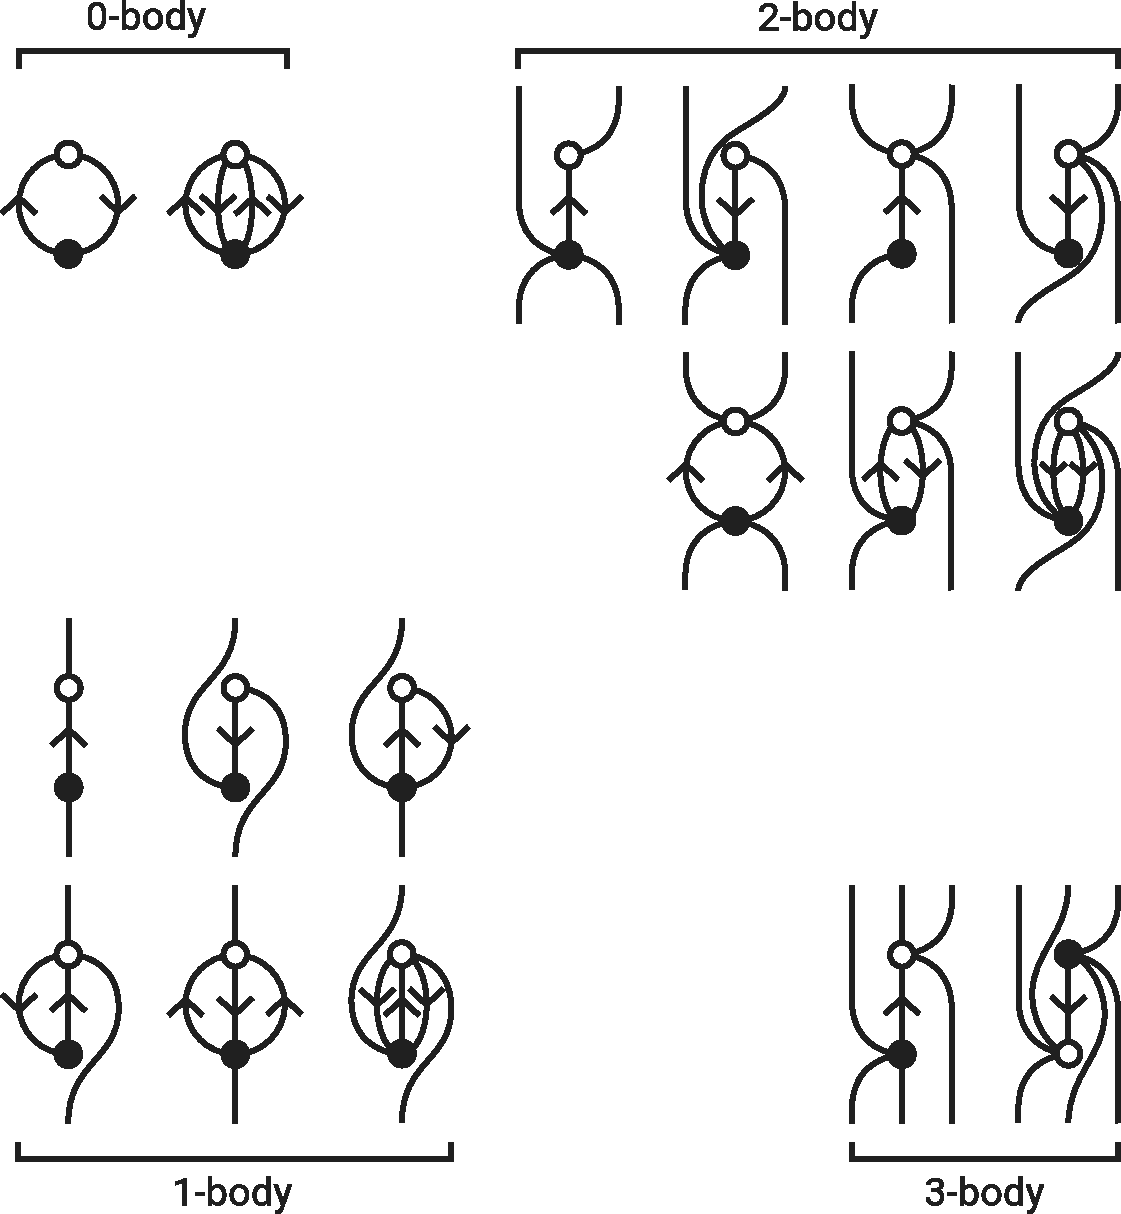
\includegraphics[width=.48\textwidth]{fig-diagrams-imsrg}
\caption{Diagrammatic form of $\hat C(\circ, \bullet)$.}
\label{fig:diagrams-imsrg}
\end{figure}
Expanding the commutator leads to the expression
\begin{align*}
  [\hat \eta, \hat H] = \hat C(\hat \eta, \hat H) - \hat C(\hat H, \hat \eta)
\end{align*}
where $\hat C$ is defined diagrammatically in Figure \ref{fig:diagrams-imsrg}.
For IM-SRG(2), we truncate the commutator to a two-body operator, neglecting
the three-body term.

\subsection{The self-energy correction}
\label{subsec:selfenergy}

IM-SRG, in the form described, does not provide a means to obtain ground state
energies of open-shell systems.  While there exists a multi-reference IM-SRG
that can handle the general problem ([[cite Heiko?]]), we opted to use a much
simpler approach to obtain the addition and removal energies: quasidegenerate
perturbation theory (QDPT).  In QDPT, the solutions of the approximate
Hamiltonian $\hat H^{\text o}$ are used as the basis of the model space.  One
then assumes the existence of an operator $\hat \Omega$, known as the
\textit{wave operator}, that maps some set of states $\tilde \Phi_u$ within
the model space to the exact ground state $\Psi_u$:
\begin{align} \label{eq:omega-condition1}
  \Psi_u = \hat \Omega \tilde \Phi_u
\end{align}
The states $\tilde \Phi_u$ consist of some mixture of the eigenstates
$\Phi_{u'}$ of the approximate Hamiltonian $\hat H^{\text o}$.

There is some freedom in the choice of the wave operator $\hat \Omega$.  We
assume it has the following form:
\begin{align} \label{eq:omega-condition2}
  \hat \Omega = \hat P + \hat Q \hat \Omega \hat P
\end{align}
where $\hat P$ projects any state into the model space and $\hat Q$ is the
complement of $\hat P$.  This entails that the exact states $\Psi_u$ is no
longer normalized but instead satisfies the typical intermediate
normalization: $\langle \Psi_u | \tilde \Phi_u \rangle = 1$.

Making use of the assumptions in Eq.\ \eqref{eq:omega-condition1} and
\eqref{eq:omega-condition2}, one can derive from the Schr\"odinger equation
the generalized Bloch equation, the main equation of QDPT:
\begin{gather*}
  [\hat \Omega, \hat H^{\text o}] =
  (1 - \hat \Omega) \hat V \Omega
\end{gather*}
where $\hat V \equiv \hat H - \hat H^{\text o}$ is the perturbation.  The
commutator on the left may be ``inverted'' using the resolvent approach
[[ShavittBartlett,p.50]], resulting in:
\begin{align*}
  \hat Q \Omega \hat P_u =
  \hat R_u (1 - \hat \Omega) \hat V \Omega \hat P_u
\end{align*}
where
$\hat R_u \equiv \hat Q (E_u - \hat Q \hat H^{\text o} \hat Q)^{-1} \hat Q$ is
the resolvent and $\hat P_u$ projects any state onto $\Phi_u$.  As is typical
in perturbation theory, we assume $\hat \Omega$ can be expanded as a series of
the increasing order as measured by the ``power'' of the perturbation
$\hat V$:
\begin{align*}
  \hat \Omega = \hat P +
  \hat Q\bigl(\hat \Omega_1 + \hat \Omega_2 + \cdots\bigr) \hat P
\end{align*}
This leads to a recursion relation of $\hat \Omega$ that enables $\hat \Omega$
to be calculated up to any order, as least in theory.  Here, we show
$\hat \Omega$ up to third order: [[double-check]]
\begin{align*}
  &\hat \Omega_1 \hat P_u = \hat R_u \hat V \hat P_u \\
  &\hat \Omega_2 \hat P_u =
    \hat R_u \biggl(
    \hat V \hat R_u
    - \sum_v \hat R_v \hat V \hat P_v
    \biggr) \hat V \hat P_u \\
  &\hat \Omega_3 \hat P_u =
    \hat R_u \biggl(
    \hat V \hat R_u \hat V \hat R_u
    - \hat V \hat R_u \sum_v \hat R_v \hat V \hat P_v \\
  &\qquad\qquad
    - \sum_v \hat R_v \hat V \hat P_v \hat V \hat R_u
    - \sum_v \hat R_v \hat V \hat R_v \hat V \hat P_v \\
  &\qquad\qquad
    + \sum_v \hat R_v \sum_w \hat R_w \hat V \hat P_w \hat V \hat P_v
    \biggr) \hat V \hat P_u
\end{align*}

[[Since the systems are all closed-shell, the
diagonal approximation can be used here to simplify the calculations.]]

\begin{figure}
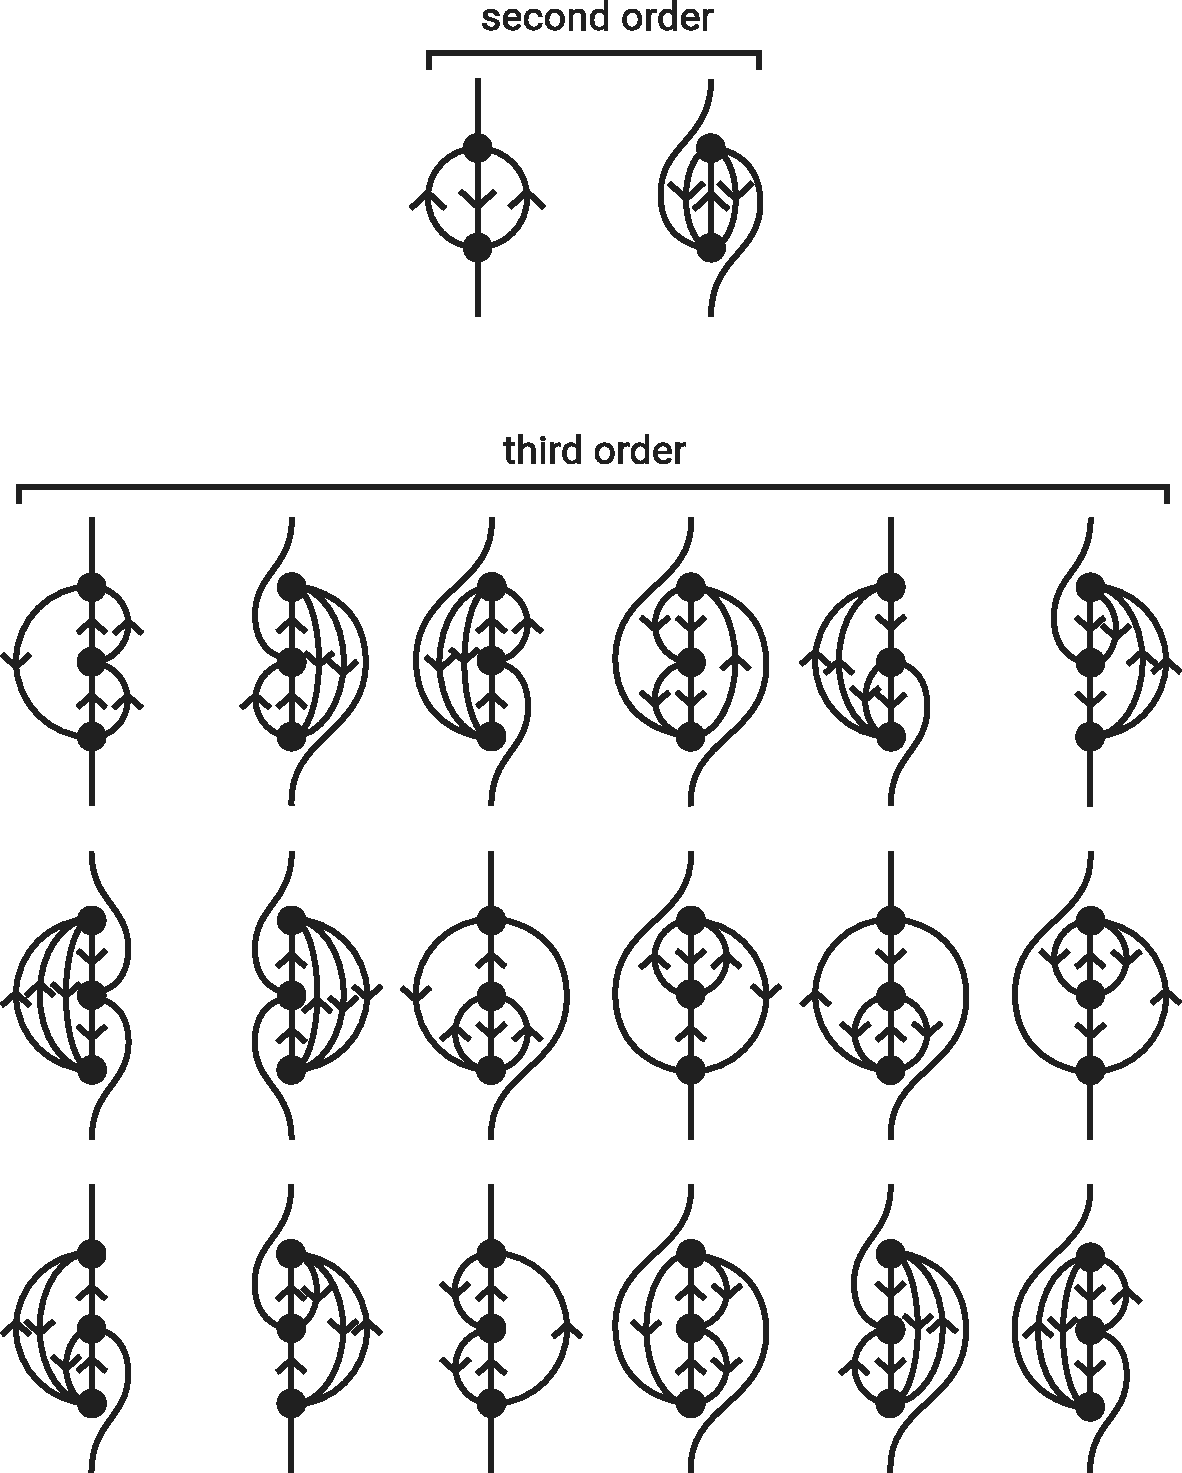
\includegraphics[width=.48\textwidth]{fig-diagrams-sfe}
\caption{Diagrammatic form of the second- and third-order self-energy
  corrections.}
\label{fig:diagrams-sfe}
\end{figure}
[[Discuss how]]
The diagrams for each order of correction can be evaluated using algebraic or
diagrammatic techniques.  The second-order correction is given by
\begin{gather*}
  \epsilon_p = \frac{1}{2} \biggl(
      \sum_{i a b} \frac{|V_{p i a b}|^2}{f_p + f_i - f_a - f_b}
    - \sum_{i j a} \frac{|V_{i j p a}|^2}{f_i + f_j - f_p - f_a}
  \biggr)
\end{gather*}
and depicted in Figure \ref{fig:diagrams-sfe}.  Since there are numerous terms in
the third-order correction, they are simply listed in a diagrammatic form in
Figure \ref{fig:diagrams-sfe}.

[[...]]

\subsection{Diffusion Monte Carlo}




Diffusion Monte Carlo (DMC) is a method for calculating the ground state
properties via a stochastic process akin to classical diffusion, refining an
approximate ground state density towards that of the exact ground state.  The
rules that govern the diffusion process are obtained by evolving the wave
function using what can be formally be thought of as the time-dependent
Schr\"odinger equation along imaginary time $t = \mathrm i \tau$:
\begin{align} \label{eq:itse}
  \frac{\partial}{\partial \tau} |\Phi(\tau)\rangle = \hat H |\Phi(\tau)\rangle
\end{align}
The solutions to this equation are not unlike the ordinary Schr\"odinger
equation with a slight but crucial difference in the exponent:
\begin{align*}
  |\Phi(\tau)\rangle = \mathrm e^{-\hat H \tau} |\Phi(0)\rangle
\end{align*}
where $|\Phi(0)\rangle$ is the initial wave function at $\tau = 0$ -- not to
be confused with the exact ground state of $\hat H$, which we denote
$|\Psi_0\rangle$ here.  If we decompose the wave function into a sum over the
eigenstates $|\Psi_n\rangle$,
\begin{align*}
  |\Psi(\tau)\rangle
  = \mathrm e^{-\hat H \tau} \sum_n c_n |\Psi_n\rangle
  = \sum_n c_n \mathrm e^{-E_n \tau} |\Psi_n\rangle
\end{align*}
we find that components of the wave function that have negative energy will
increase exponentially as $\tau \to \infty$, while those with positive energy
will decrease exponentially.  This property can be exploited to filter out the
undesirable components, leaving only the ground state energy.  To do this, we
require a trial energy $E_{\text{T}}$ -- a guess of the ground state energy --
and replace $\hat H$ in \eqref{eq:itse} with $(\hat H - E_{\text{T}})$ so
that, if our trial energy is good, all states but the ground states will
approximately vanish.

Diffusion Monte-Carlo (DMC) is a method used for refining a crude estimate to the ground state density into a better approximation to the exact ground state. The basic idea is to move multiple random walkers in position space with sampling rules which ensures convergence to a behavior representing a walk guided by the exact ground state density. Once a satisfying level of convergence is reached, expectation values are calculated by accumulating local estimates along the path of the walkers.

The equations representing the DMC algorithm is obtained by applying the projection operator $\OP{P}(\tau)$ on the crude trial state $\ket{\Psi_T}$
\begin{equation}
 \OP{P}(\tau)\ket{\Psi_T} \equiv \exp\left({-(\OP{H} - E_0)\tau}\right)\ket{\Psi_T} 
\end{equation}
\noindent
where $\tau$ is a constant often described as imaginary time, and $E_0=\bra{\Psi_0}\OP{H}\ket{\Psi_0}$ is the ground state of the Hamiltonian $\OP{H}$. By expanding the trial state in the eigenfunctions of $\OP{H}$, the ground state is obtained up to a constant factor

\begin{equation}
 \label{eq:DMC_ExactProjection}
 \lim_{\tau\to\infty} \bra{\mathbf{r}}  \OP{P}(\tau) \ket{\Psi_T} = \braket{\Psi_0}{\Psi_T}\Psi_0(\mathbf{r}).
\end{equation}

Defining $\Phi(\mathbf{r}, \tau) \equiv \bra{\mathbf{r}}\OP{P}(\tau)\ket{\Psi_T}$, we obtain the state at a later time $\tau + \delta\tau$ through projection

\begin{align}
 \Phi(\mathbf{r}, \tau + \delta\tau) &= \bra{\mathbf{r}} P(\tau + \delta\tau) \ket{\Psi_T} \notag\\
 &= \bra{\mathbf{r}} \exp\left({-(\OP{H} - E_0)\delta\tau}\right) \OP{P}(\tau) \ket{\Psi_T} \notag\\
 &= \bra{\mathbf{r}} \exp\left({-(\OP{H} - E_0)\delta\tau}\right) \ket{\Phi(\tau)} \notag\\
 &= \int \mathrm{d}\mathbf{r}' \bra{\mathbf{r}} \exp\left({-(\OP{H} - E_0)\delta\tau}\right)\ket{\mathbf{r}'} \Phi(\mathbf{r}', \tau)\notag \\
 &\equiv \int \mathrm{d}\mathbf{r}' G(\mathbf{r}, \mathbf{r}'; \delta\tau) \Phi(\mathbf{r}', \tau). \label{eq:DMC_GreenFuncRevealed}
\end{align}

In practice, the ground state energy is a priori unknown, hence a trailing averaged value obtained from the converging DMC density is used. This energy is often referred to as the trial energy, and it is believed that with a sufficiently good trial state, the error due to this approximation is small.

The Green's function introduced in Eq.~(\ref{eq:DMC_GreenFuncRevealed}) has singularities due to the the Coulomb interaction term in $\OP{H}$. Due to Pauli exclusion these are not physical, nevertheless, in numerical implementations they are unpredictable and undesirable, hence we want to avoid them. 

For evaluation of the local energy, the trial state is designed to cancel the Coulomb singularities by containing so-called correlation factors, however, this cancellation does not apply to the terms in the Green's function. In order to transfer this behavior to apply to the Green's function, a change to the formalism is introduced by iterating on a mixed density $f(\mathbf{r}, \tau) \equiv \Phi(\mathbf{r}, \tau)\Psi_T(\mathbf{r})$. Note that all previous arguments regarding convergence to the true ground state still applies for the new distribution. 

Methods exist for transforming the mixed density into the pure density $|\Phi(\mathbf{r}, \tau)|^2$ \cite{abInitioMC}, but unless the pure density is explicitly needed (e.g.~for comparisons with other methods), this is strictly not necessary.

Additionally, to avoid issues regarding the positive definiteness of the mixed distribution, the nodes of the mixed density is fixed to those of the wave function of the trial state. This is known as the \textit{fixed node approximation} \cite{umrigar:2865, abInitioMC}. Again, given a sufficiently good trial state, the errors should be small.

The Green's function for the mixed density is given as \cite{umrigar:2865}

\begin{align}
  G(\mathbf{r}, \mathbf{r}'; \delta\tau)_f &= \bra{\mathbf{r}} \exp\left({\frac{1}{2}\nabla\cdot \left[\left(\nabla - \mathbf{F}(\mathbf{r})\right)\right] - \left(E_L(\mathbf{r}) - E_T\right)}\right)\ket{\mathbf{r}'} \label{eq:DMC_IS_GF_raw}\\
  &\propto e^{-\left[|\mathbf{r} - \mathbf{r}' - \frac{1}{2}\delta\tau\mathbf{F}(\mathbf{r})|^2/2\delta\tau\right]} \label{eq:DMC_IS_GF}\\
  &\qquad\times e^{-\left[\frac{1}{2}\left[E_L(\mathbf{r'}) + E_L(\mathbf{r})\right] - E_T\right]\delta\tau} + \mathcal{O}(\delta\tau^2), \notag
\end{align}
where 
\begin{equation}
  \mathbf{F}(\mathbf{r}) = 2\Psi_T(\mathbf{r})^{-1} \nabla \Psi_T(\mathbf{r})
\end{equation}

\noindent
is the drift vector commonly referred to as the \textit{quantum force}.

The local energy 
\begin{equation} 
E_L(\mathbf{r}) = \Psi_T(\mathbf{r})^{-1}\OP{H} \Psi_T(\mathbf{r})
\end{equation} 
is necessarily sampled from $|\Psi_T(\mathbf{r})|^2$ (ensured by using the Metropolis Algorithm \cite{abInitioMC}) to avoid undefined energies when sampling close to the nodes of $\Psi_T(\mathbf{r})$.

The Green's function from Eq.~(\ref{DMC_IS_GF_raw}) has been split into two for practical reasons; one part containing the kinetic terms, more specifically this represents a Fokker-Planck diffusion process, and a second part which is commonly referred to as a \textit{branching function}, which is an effective reweighing of a positions contribution to the overall density. Excluding branching we will simply sample from the density of the trial state.

In order dampen the errors introduced by splitting the Green's function, the time step $\delta\tau$ should be small. A value in the range of $10^{-3}$ to $10^{-4}$ is used in this work. High variance in energy samples requires a smaller time step to keep the branching controlled, since the fluctuations of the two are connected by Eq.~(\ref{eq:DMC_IS_GF}).

The name branching arise from the fact that in DMC, the weights are implemented as a probability of a given walker to copy or delete itself $n$ times, where $\langle n \rangle$ equals the branching term of Eq.~(\ref{eq:DMC_IS_GF}). Let $G_b$ denote the value of the branching function at a given position. Correct weighting is then ensured by guaranteeing $m = \max\left(\mathrm{floor}\left(G_b\right)-1, 0\right)$ branches with a probability $G_b - m$ of getting an additional branch. A branch is an identical copy of the corresponding walker, with an identical past but with a different future. When the number of requested branches is zero, the walker is removed from the simulation.


Initially, $N_w$ walkers are initialized to span $|\Psi_T(\mathbf{r})|^2$. This is ensured by using the Metropolis Algorithm. Moreover, importance sampling is ensured by sampling according to the kinetic term of  Eq.~(\ref{eq:DMC_IS_GF_raw}) \textit{cite solution langevin}

\begin{equation}
x_{i+1} = x_i + \frac{1}{2}\delta\tau F(\mathbf{r})_x + \xi,
\end{equation}
\noindent
where $\xi$ is a uniform distributed random number with variance $\mathrm{Var}(\xi) = 2D\delta\tau$. A typical value of $N_w$ in this work is 250 000.

For each time step, diffusion and branching repeats a given number of blocks $N_b$ for each walker. New branches are not active until the next time step, and if a walker hits zero branches the block repetition stops. During these block loops, the trial energy $E_T$ is sampled for use in the next time step $k+1$

\begin{equation}
 E_T^{k+1} = \frac{1}{M^{(k)}}\sum_{i=1}^{M^{(k)}} G_b(\mathbf{r}^{(k)}_i)E_L(\mathbf{r}^{(k)}_i),
\end{equation}
\noindent
where $M^{(k)}$ is the total number of samples obtained in cycle $k$. For this work we have found a value of $N_b = 100$ to be sufficient. 

Several methods for estimating $E_0$ exist in the literature, one of which is simply an average of all $N_c$ trial energies calculated after $N_t$ thermalization cycles 
\begin{equation}
 E_0 = \frac{1}{N_c-N_t}\sum\limits_{k=N_t}^{N_c} E_T^{(k)}.
\end{equation}
This is the relation we use in this work to obtain the DMC energies.

In this work, the trial state has been chosen to consist of a single Slater determinant (cite) 
together with a single variational parameter Padé-Jastrow correlation function (cite). 

The Slater determinant contains eigenstates $\phi_n(\mathbf{r})$ of Eq.~(\ref{eq:potential})
with a variational parameter $\alpha$ scaling the oscillator frequency $\omega$ 
such that $\omega\to\alpha\omega$ in all solutions:

\begin{equation}
 \phi_n(\mathbf{r}) = H_n(\sqrt{\alpha\omega}x)H_n(\sqrt{\alpha\omega}y)\exp(-\alpha\omega r^2),
\end{equation}

\noindent
where $H_n$ is the $n$'th level Hermite polynomial.


The eigenstates are selected such that the $N$ lowest lying energy eigenstates are selected (counting spin-degeneracy). Due to the Hamiltonian being spin independent we may split the Slater determinant into two equal parts - 
one for each spin level (cite). The overall form of the trial state is as follows:

\begin{equation}
 \Psi_T(\mathbf{r}) = S(\mathbf{r}^\uparrow) S(\mathbf{r}^\downarrow) \prod_{i<j}^{N} J(r_{ij}),
\end{equation}

with

\begin{equation}
 S(\mathbf{r}^s) =  \left| \begin{array}{cccc}
\phi_1(\mathbf{r}^s_1) & \phi_2(\mathbf{r}^s_1)& \cdots & \phi_\frac{N}{2}(\mathbf{r}^s_1) \\
\phi_1(\mathbf{r}^s_2) & \phi_2(\mathbf{r}^s_2)& \cdots & \phi_\frac{N}{2}(\mathbf{r}^s_2) \\
\vdots & \vdots& \ddots & \vdots \\
\phi_1(\mathbf{r}^s_\frac{N}{2}) & \phi_2(\mathbf{r}^s_\frac{N}{2})& \cdots & \phi_\frac{N}{2}(\mathbf{r}^s_\frac{N}{2}) \\
 \end{array} \right|,
\end{equation}

and 

\begin{equation}
 J(r_{ij}) = \exp\left(\frac{r_{ij}}{1 + \beta r_{ij}}\right),
\end{equation}

where $\mathbf{r}^s_i$ denotes $i$'th particle with spin $s$, and $r_{ij}$ is the relative distance between two electrons. 
Since Metropolis Monte-Carlo only involves ratios of density functions, all normalization factors are skipped.

As a consequence of the variational principle, the optimal numeric values for $\alpha$ and $\beta$ can be found by minimizing the energy in the variational parameter space.
For this we have used the adaptive step gradient descent method (cite ASGD).

Using a single Slater determinant and a single variational parameter in the correlation function might at first glance seem insufficient,
however, the strength and robustness of DMC greatly succeeds at transforming this naive approximation into a very good estimate to the ground
state density. It should be mentioned that for systems where the single-particle Hamiltonian does not have analytical solutions, this approach
will indeed be insufficient due to low overlap between the initial and exact state.

A single Slater determinant and a simple correlation function opens up numerous optimization schemes which trivializes the CPU-time of most calculations.
We refer to Refs (cite optimization techniques) for more information. 
Moreover, the most costly part of evaluating the single-particle eigenstates, the exponentials, is independent of the quantum number $n$, and can thus be tabulated once
for the entire calculation. This holds for the gradient and Laplacian needed in the quantum force and local energy, respectively, since the exponential shape is 
preserved under differentiation.



\section{Results}
\label{sec:results}

\begin{figure}%[hbtp]
     \begin{center}
        \subfigure[Results for $N=6$ and $\omega=1.0$ ]{
            \label{fig:N6hw1}
            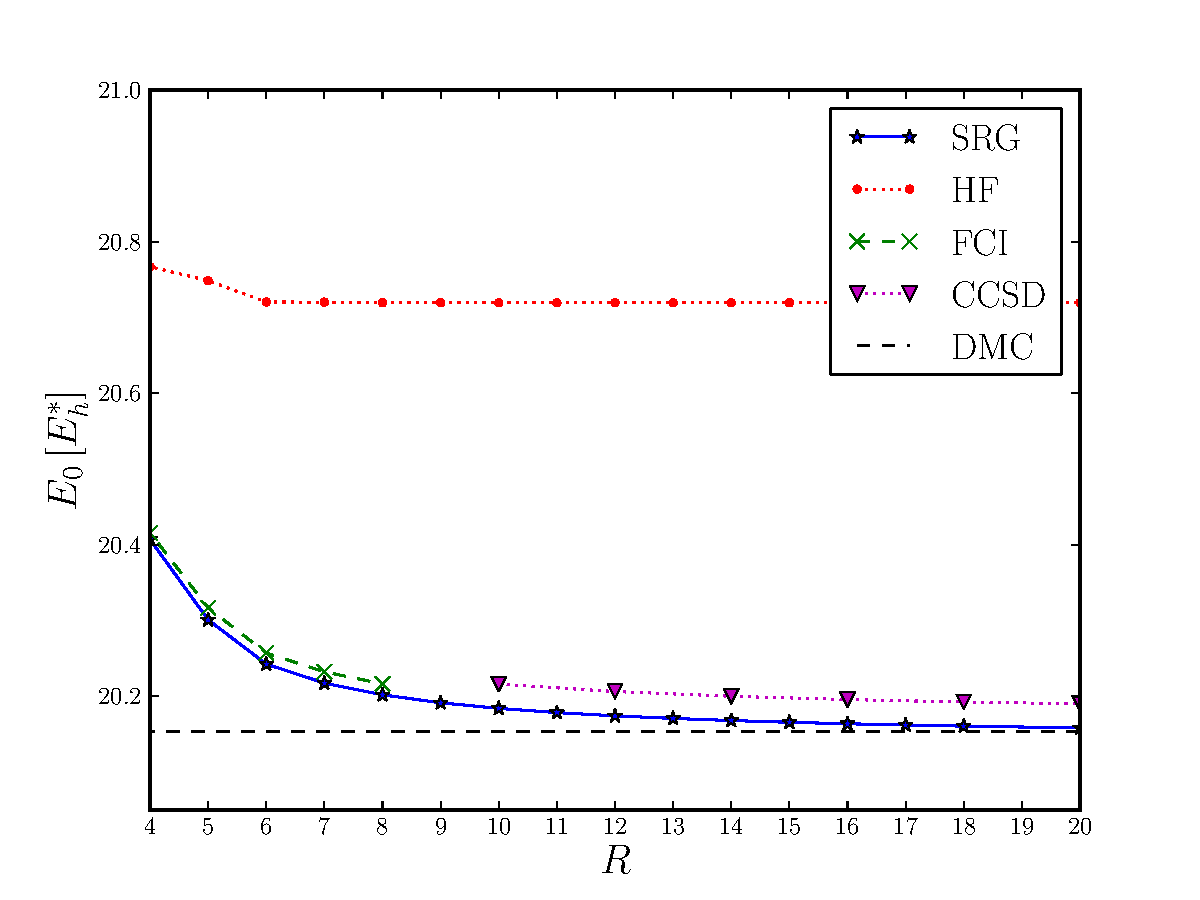
\includegraphics[width=0.38\textwidth]{figures/6parthw1.pdf}
        }
        \subfigure[Results for $N=6$ and $\omega=0.5$ ]{
           \label{fig:N6hw05}
           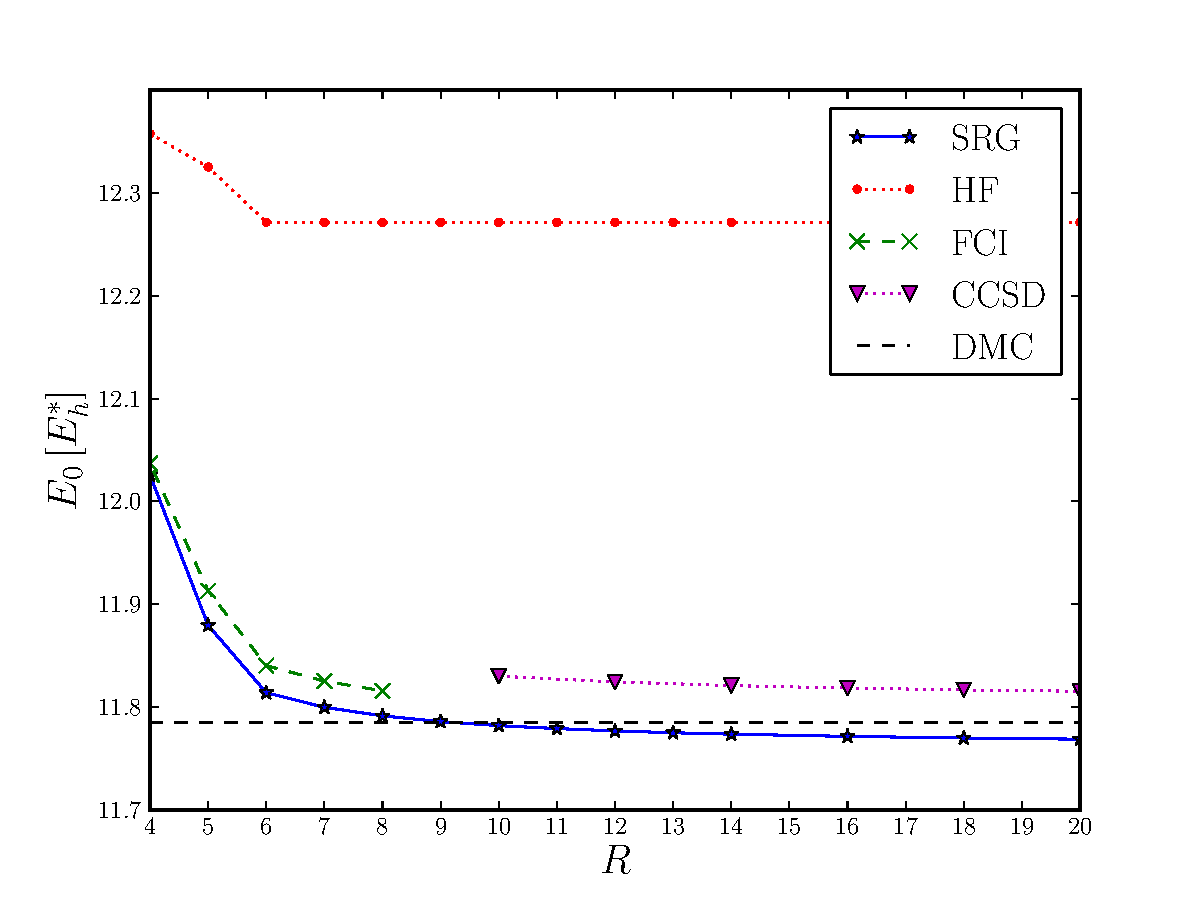
\includegraphics[width=0.38\textwidth]{figures/6parthw05.pdf}
        }\\ %  ------- End of the first row ----------------------%
        \subfigure[Results for $N=6$ and $\omega=0.28$ ]{
            \label{fig:N6hw028}
            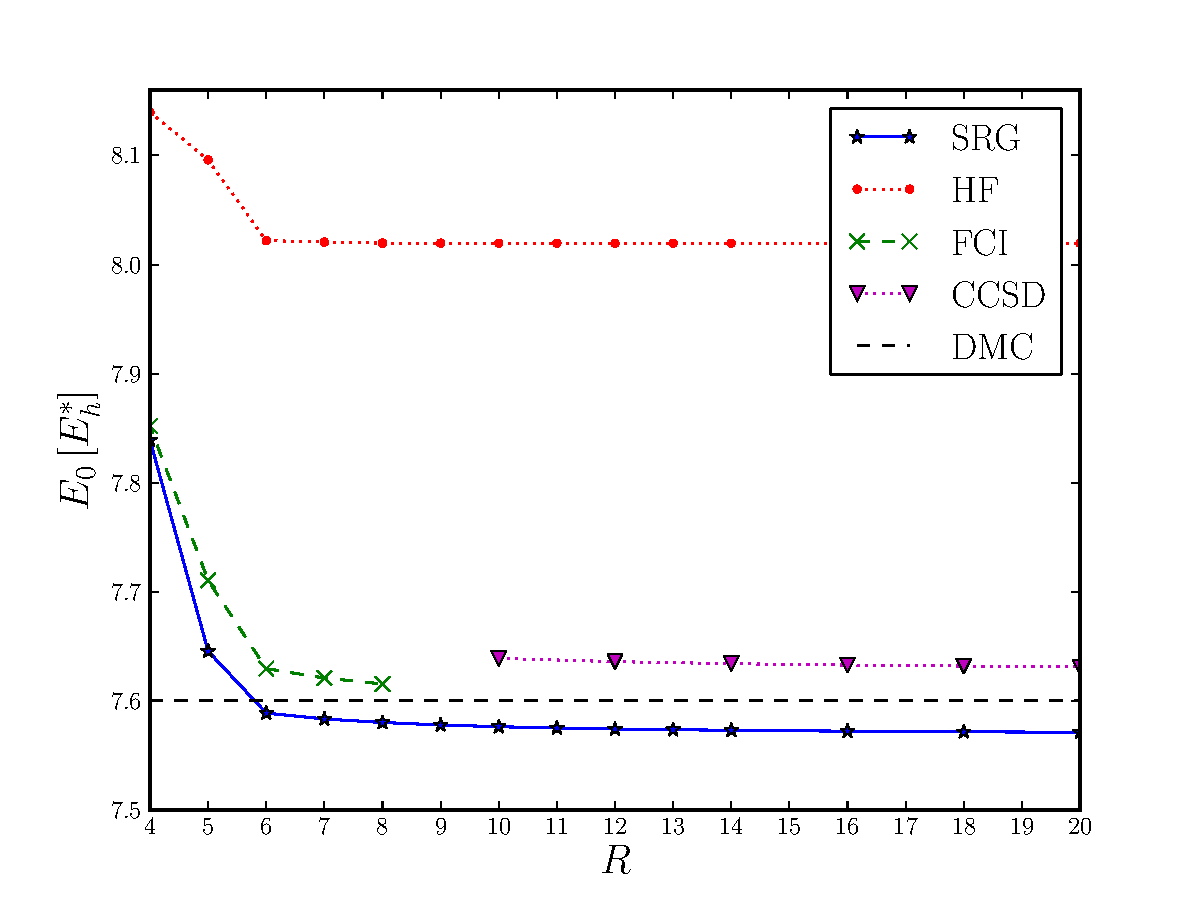
\includegraphics[width=0.38\textwidth]{figures/6parthw028.pdf}
        }
        \subfigure[Results for $N=6$ and $\omega=0.1$ ]{
            \label{fig:N6hw01}
            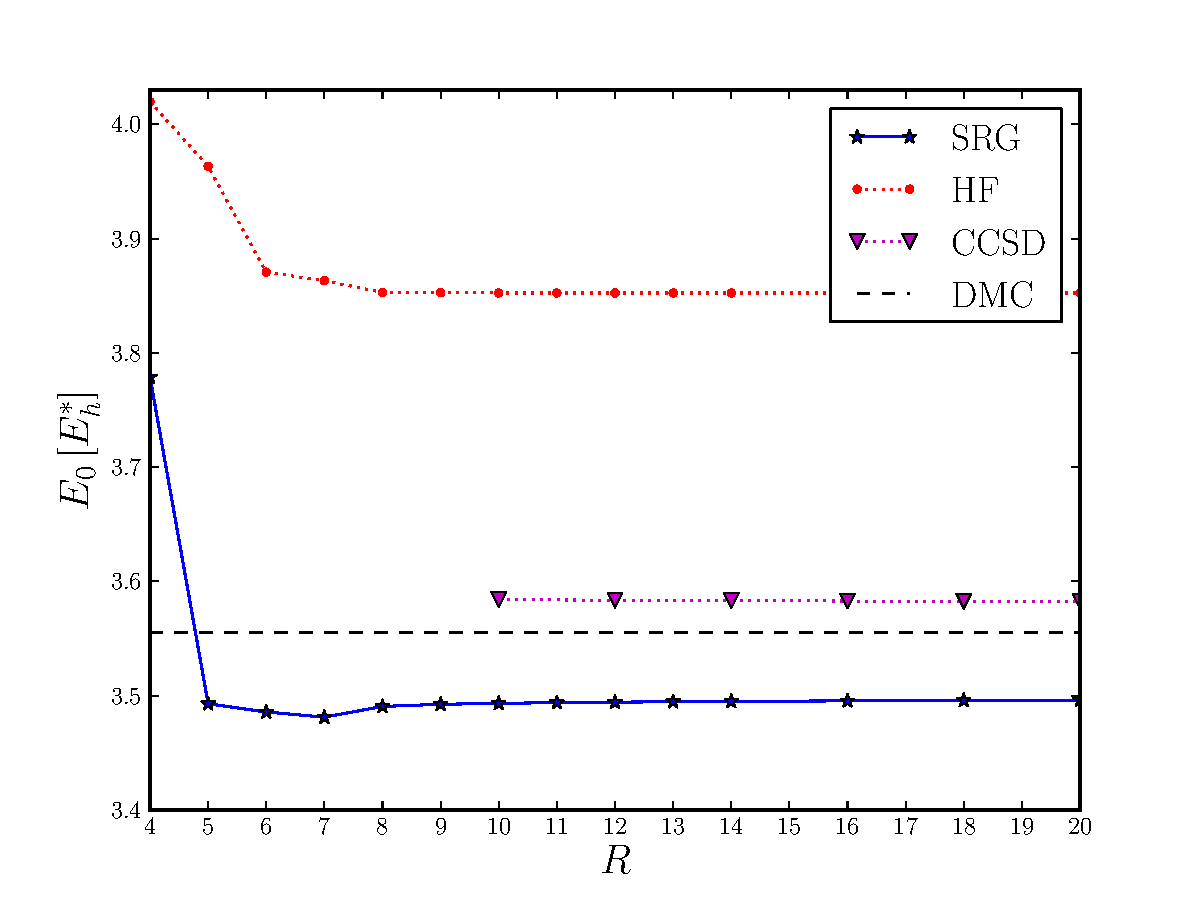
\includegraphics[width=0.38\textwidth]{figures/6parthw01.pdf}
        }
    \end{center}
    \caption{Comparison of our IM-SRG(2) ground state energies (SRG)
      for circular quantum dots for $N=6$ and $\omega=1.0$
       The results are compared with diffusion Monte Carlo (DMC),
      coupled cluster at the level of singles and doubles (CCSD), full
      configuration interaction (FCI) and Hartree-Fock calculations
      (HF) as functions of the number of major oscillator shells
      $R$. A harmonic oscilaltor basis has been used, with an
      unrenormalized Coulomb repulsion and White's generator. All
      energies in atomic units.}
   \label{fig:N6}
\end{figure}





\begin{figure}%[hbtp]
     \begin{center}
        \subfigure[Results for $N=12$ and $\omega=1.0$ ]{
            \label{fig:N12hw1}
            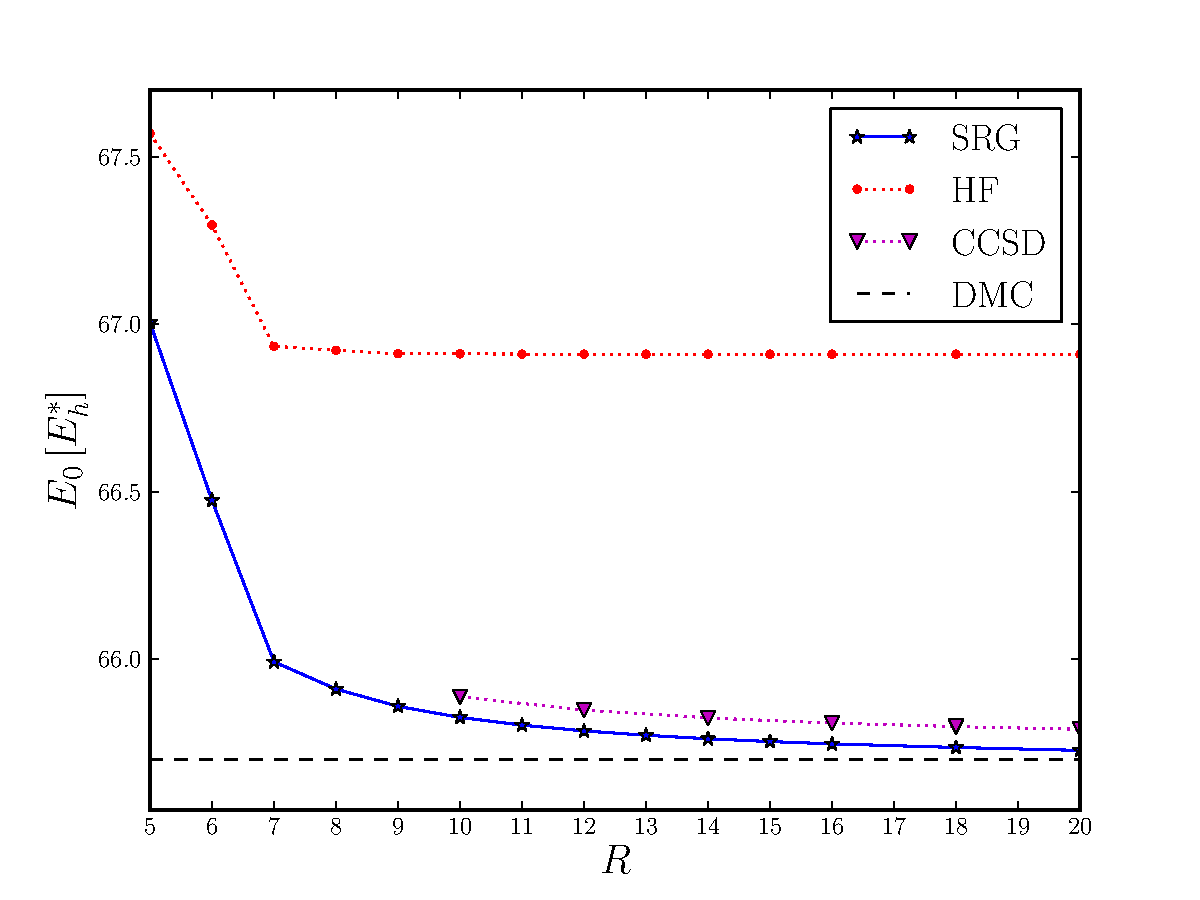
\includegraphics[width=0.38\textwidth]{figures/12parthw1.pdf}
        }
        \subfigure[Results for $N=12$ and $\omega=0.5$ ]{
           \label{fig:N12hw05}
           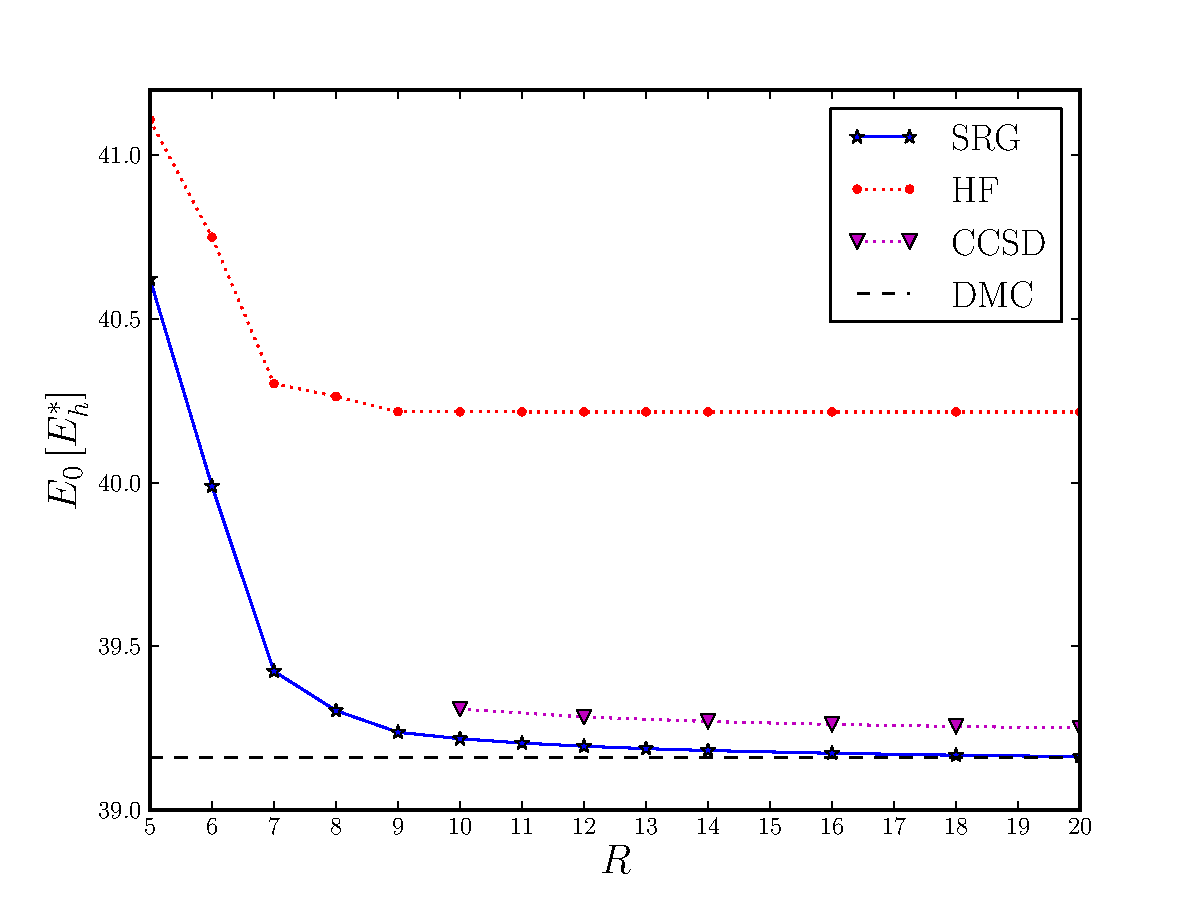
\includegraphics[width=0.38\textwidth]{figures/12parthw05.pdf}
        }\\ %  ------- End of the first row ----------------------%
        \subfigure[Results for $N=12$ and $\omega=0.28$ ]{
            \label{fig:N12hw028}
            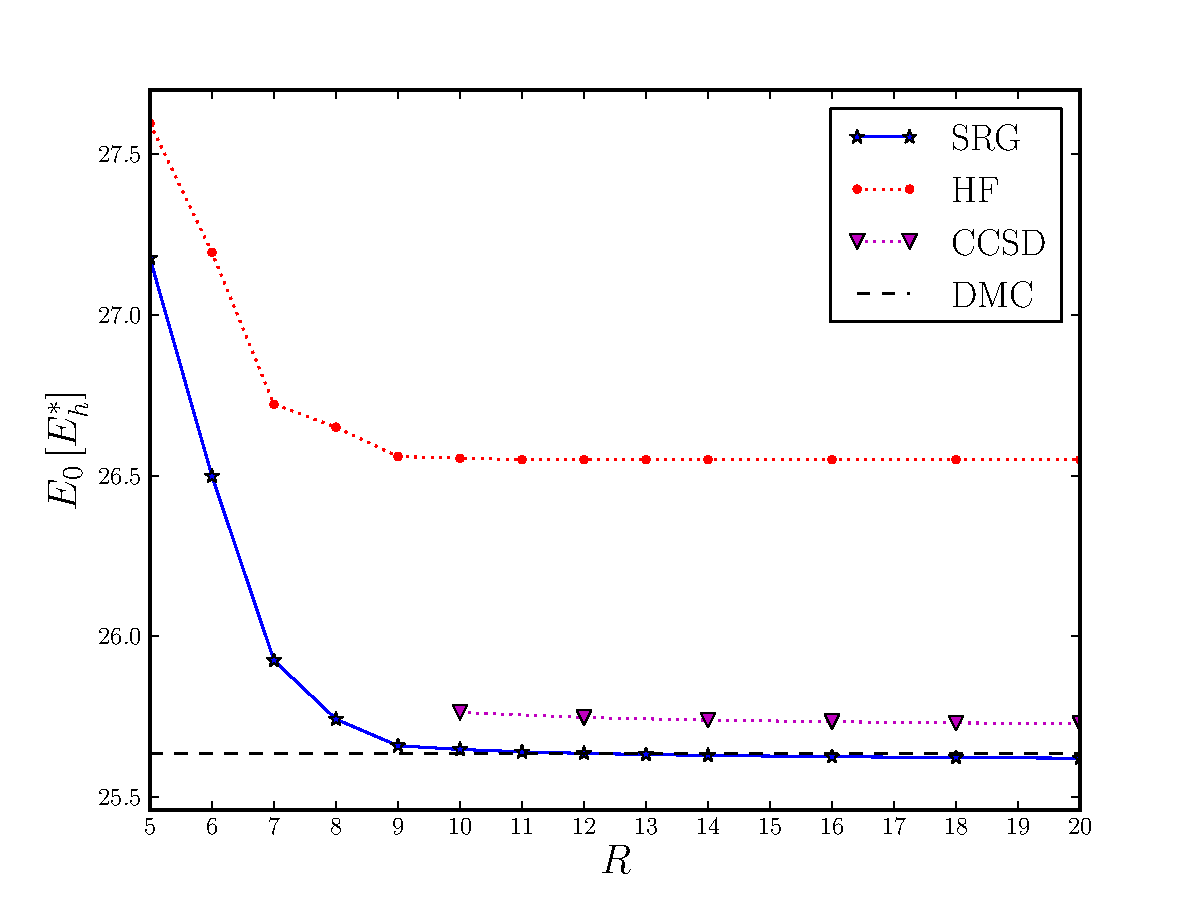
\includegraphics[width=0.38\textwidth]{figures/12parthw028.pdf}
        }
        \subfigure[Results for $N=12$ and $\omega=0.1$ ]{
            \label{fig:N12hw01}
            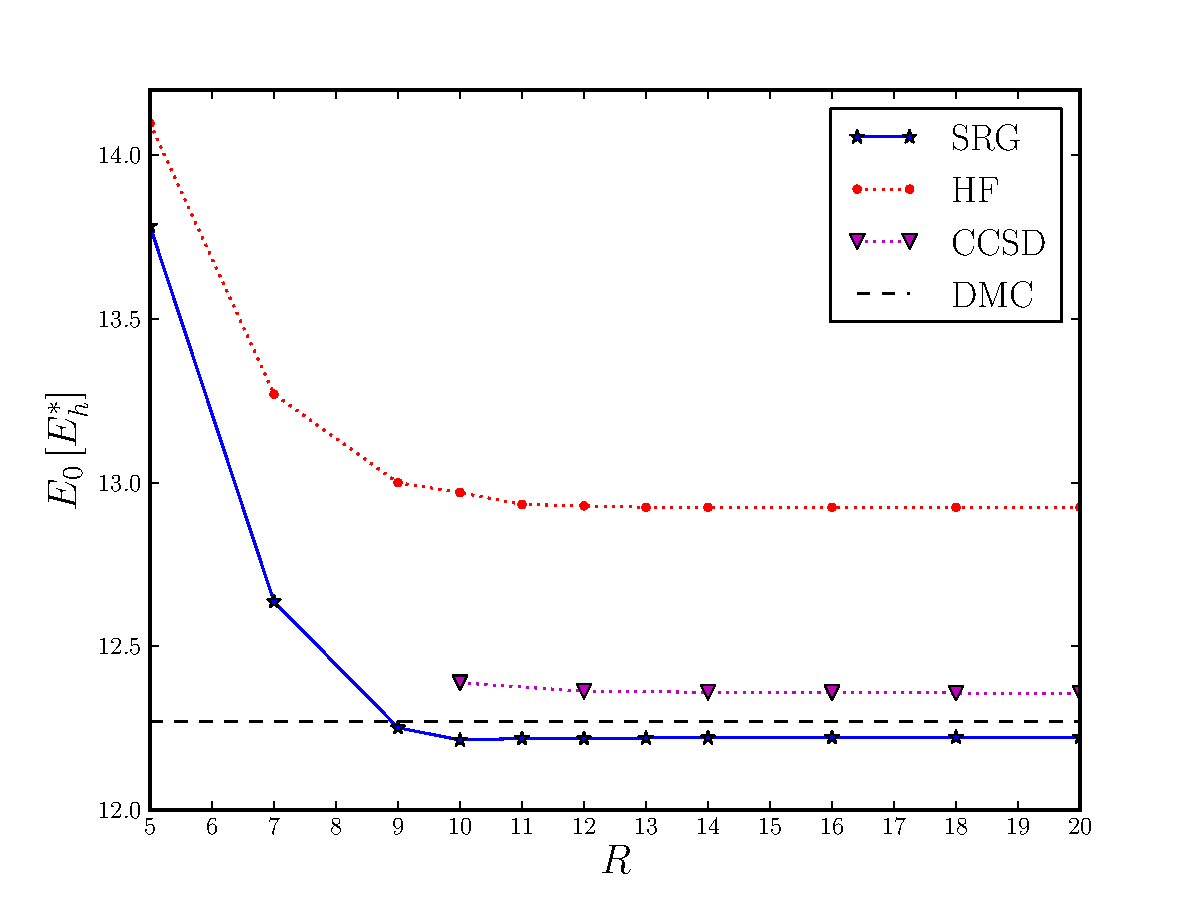
\includegraphics[width=0.38\textwidth]{figures/12parthw01.pdf}
        }
    \end{center}
    \caption{Comparison of our IM-SRG(2) ground state energies (SRG)
      for circular quantum dots for $N=12$ and different values of
      $\omega$. The results are compared with diffusion Monte
      Carlo (DMC), coupled cluster at the level of singles and doubles
      (CCSD), full configuration interaction (FCI) and Hartree-Fock
      calculations (HF) as functions of the number of major oscillator
      shells $R$. A harmonic oscilaltor basis has been used, with an
      unrenormalized Coulomb repulsion and White's generator. All
      energies in atomic units.}
   \label{fig:N12}
\end{figure}





\begin{figure}%[hbtp]
     \begin{center}
        \subfigure[Results for $N=20$ and $\omega=1.0$ ]{
            \label{fig:N20hw1}
            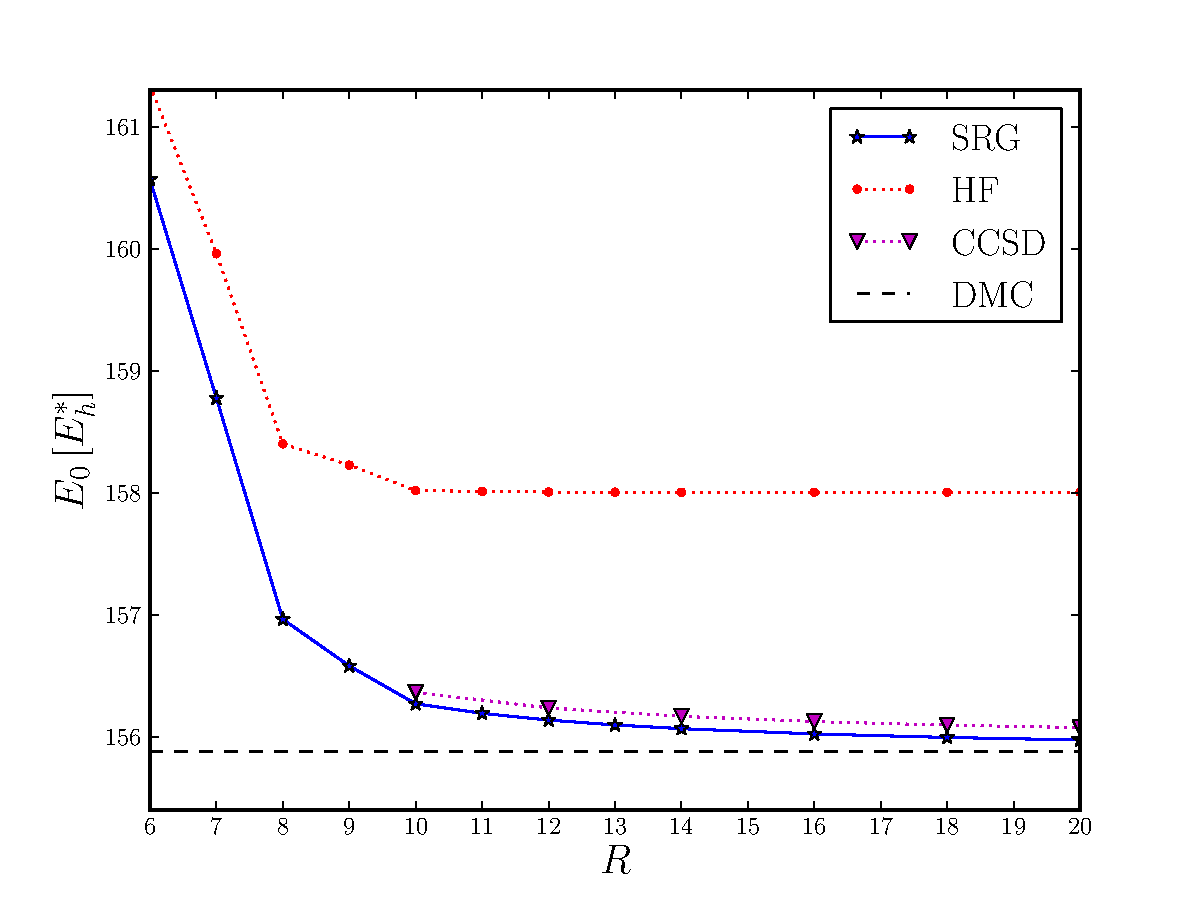
\includegraphics[width=0.38\textwidth]{figures/20parthw1.pdf}
        } \subfigure[Results for $N=20$ and $\omega=0.5$ ]{
           \label{fig:N20hw05}
           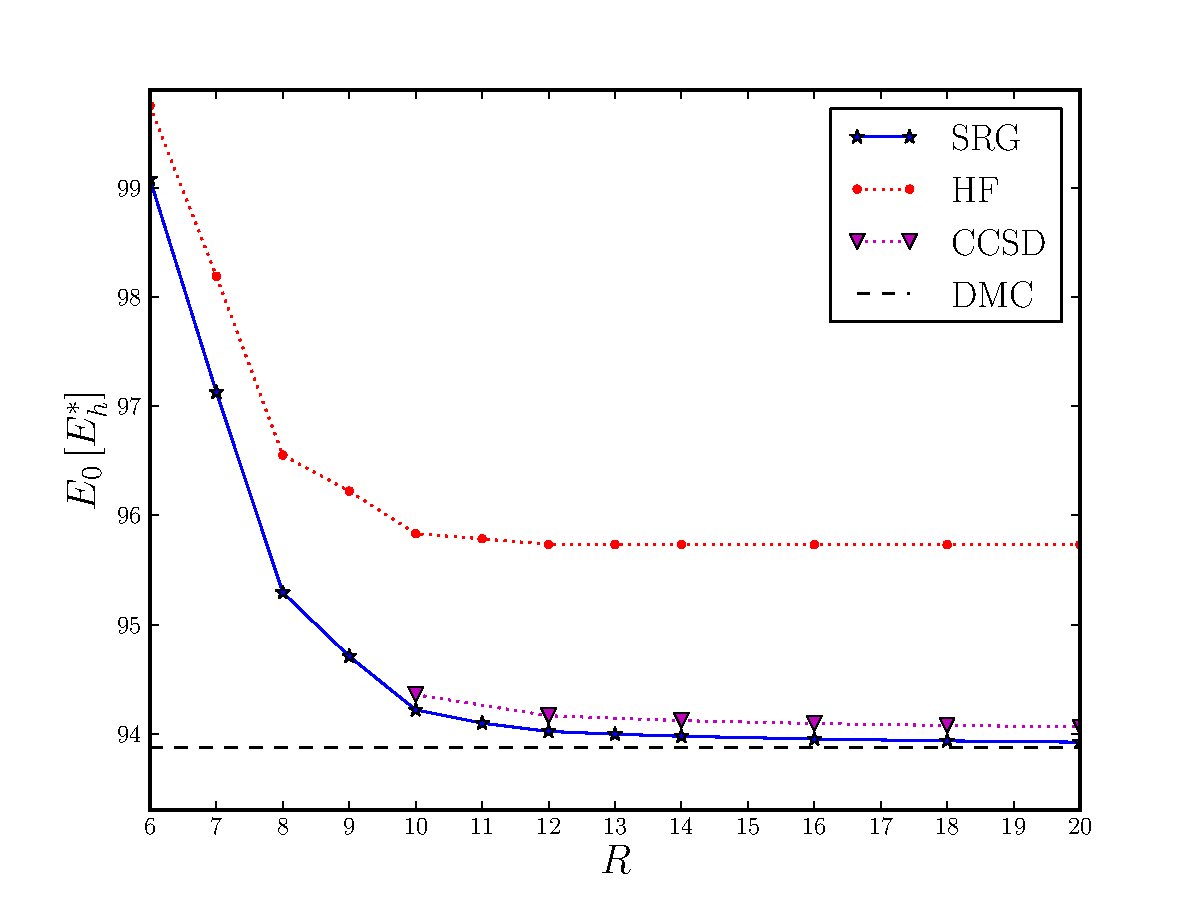
\includegraphics[width=0.38\textwidth]{figures/20parthw05.pdf}
        }\\ % ------- End of the first row ----------------------%
        \subfigure[Results for $N=20$ and $\omega=0.28$ ]{
            \label{fig:N20hw028}
            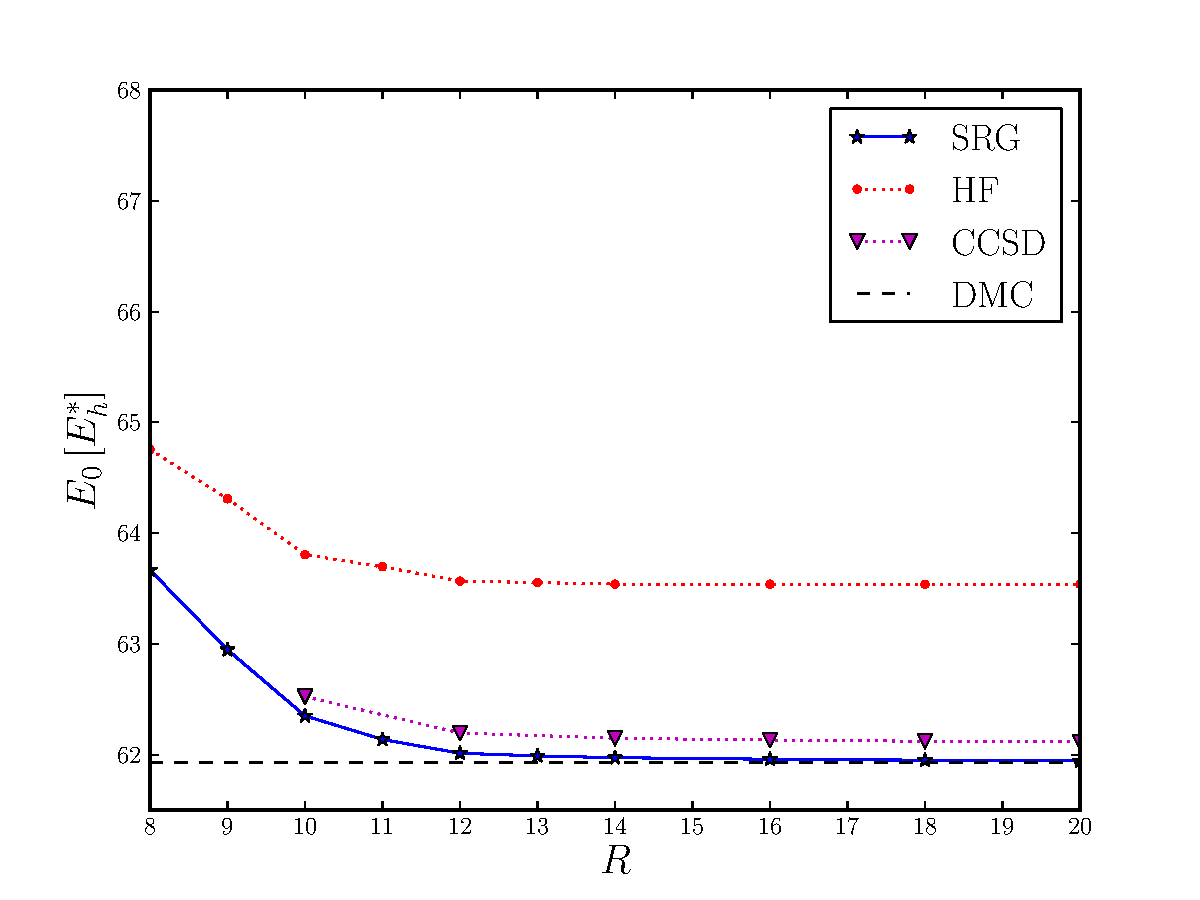
\includegraphics[width=0.38\textwidth]{figures/20parthw028.pdf}
        } \subfigure[Results for $N=20$ and $\omega=0.1$ ]{
            \label{fig:N20hw01}
            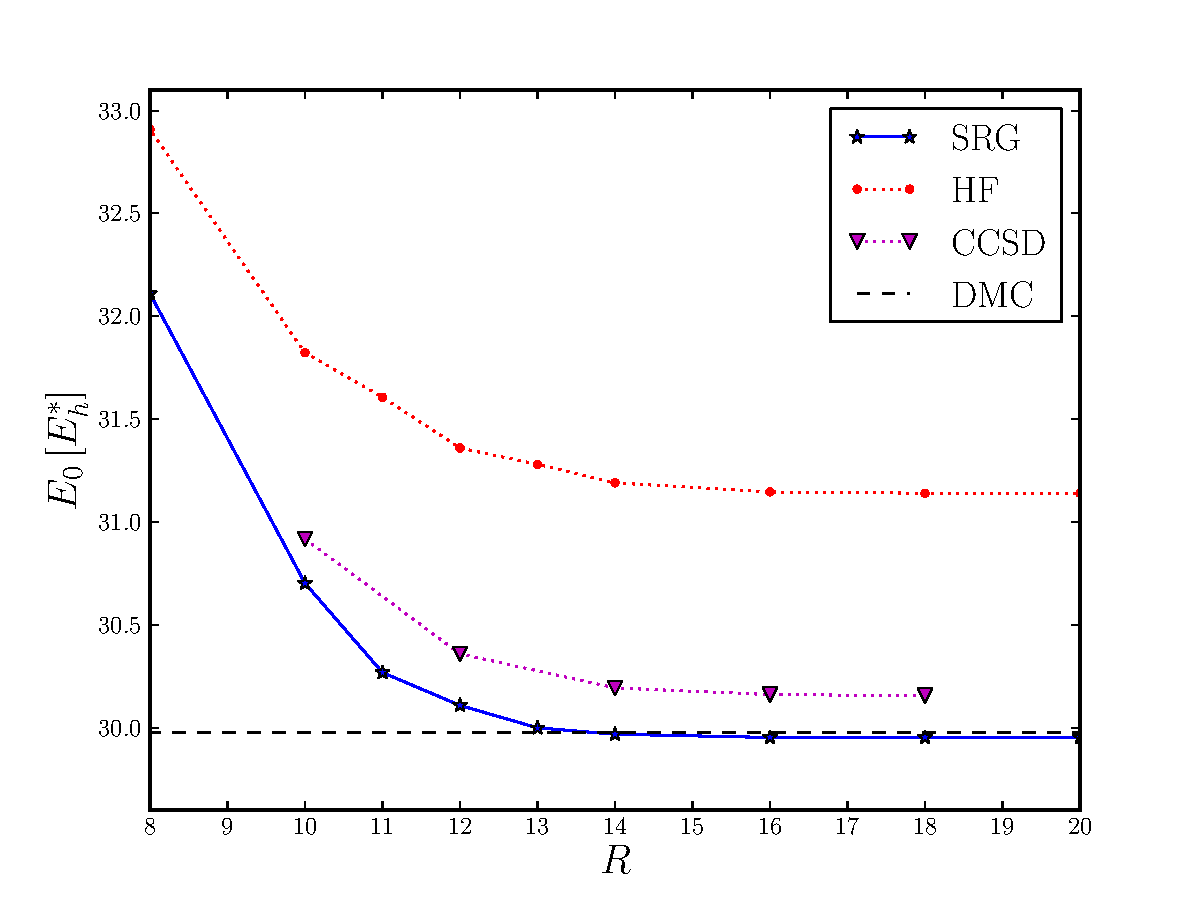
\includegraphics[width=0.38\textwidth]{figures/20parthw01.pdf}
        }
    \end{center}
    \caption{Comparison of our IM-SRG(2) ground state energies (SRG)
      for circular quantum dots for $N=20$ and different values of
      $\omega$. The results are compared with diffusion Monte
      Carlo (DMC), coupled cluster at the level of singles and doubles
      (CCSD), full configuration interaction (FCI) and Hartree-Fock
      calculations (HF) as functions of the number of major oscillator
      shells $R$. A harmonic oscilaltor basis has been used, with an
      unrenormalized Coulomb repulsion and White's generator. All
      energies in atomic units.}
   \label{fig:N20}
\end{figure}



\begin{figure}%[hbtp]
     \begin{center}
        \subfigure[Results for $N=30$ and $\omega=1.0$ ]{
            \label{fig:N30hw1}
            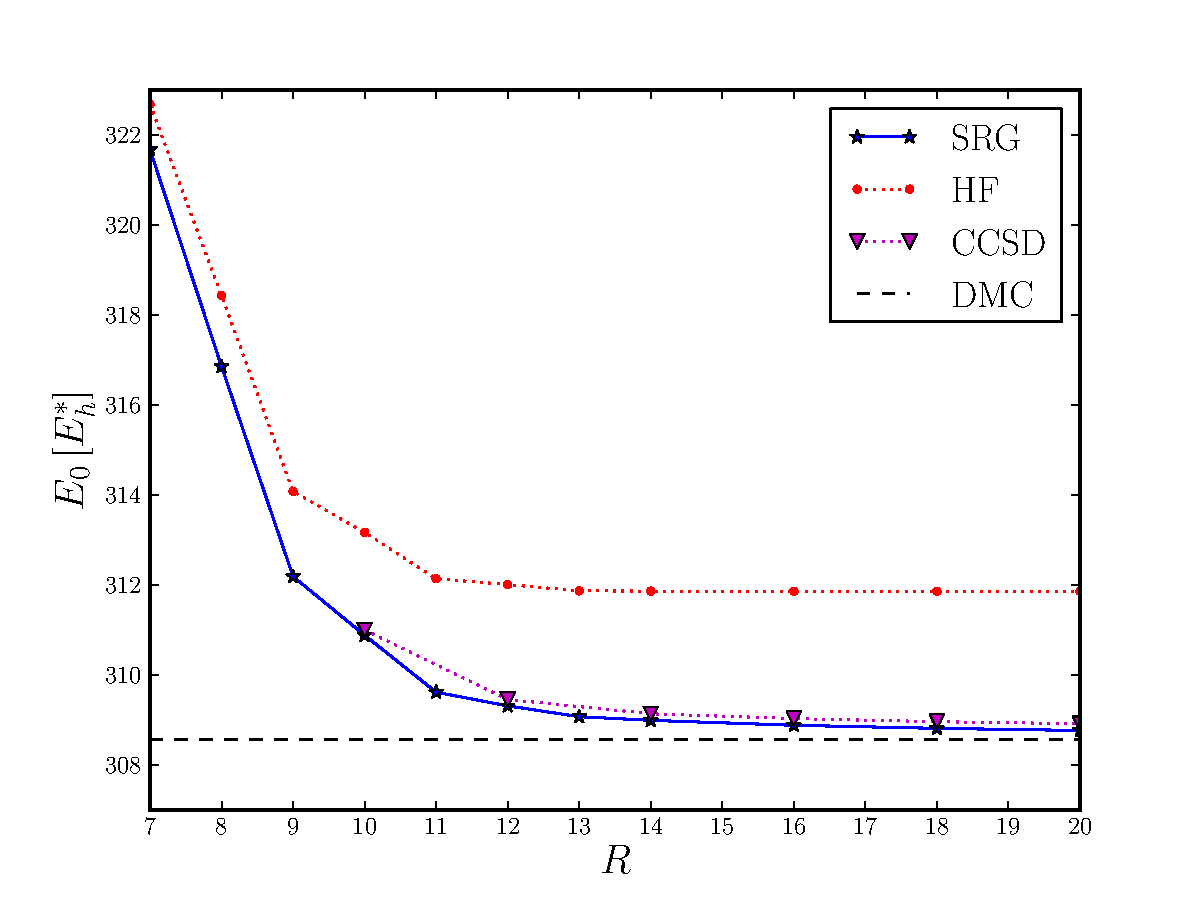
\includegraphics[width=0.38\textwidth]{figures/30parthw1.pdf}
        } \subfigure[Results for $N=30$ and $\omega=0.5$ ]{
           \label{fig:N30hw05}
           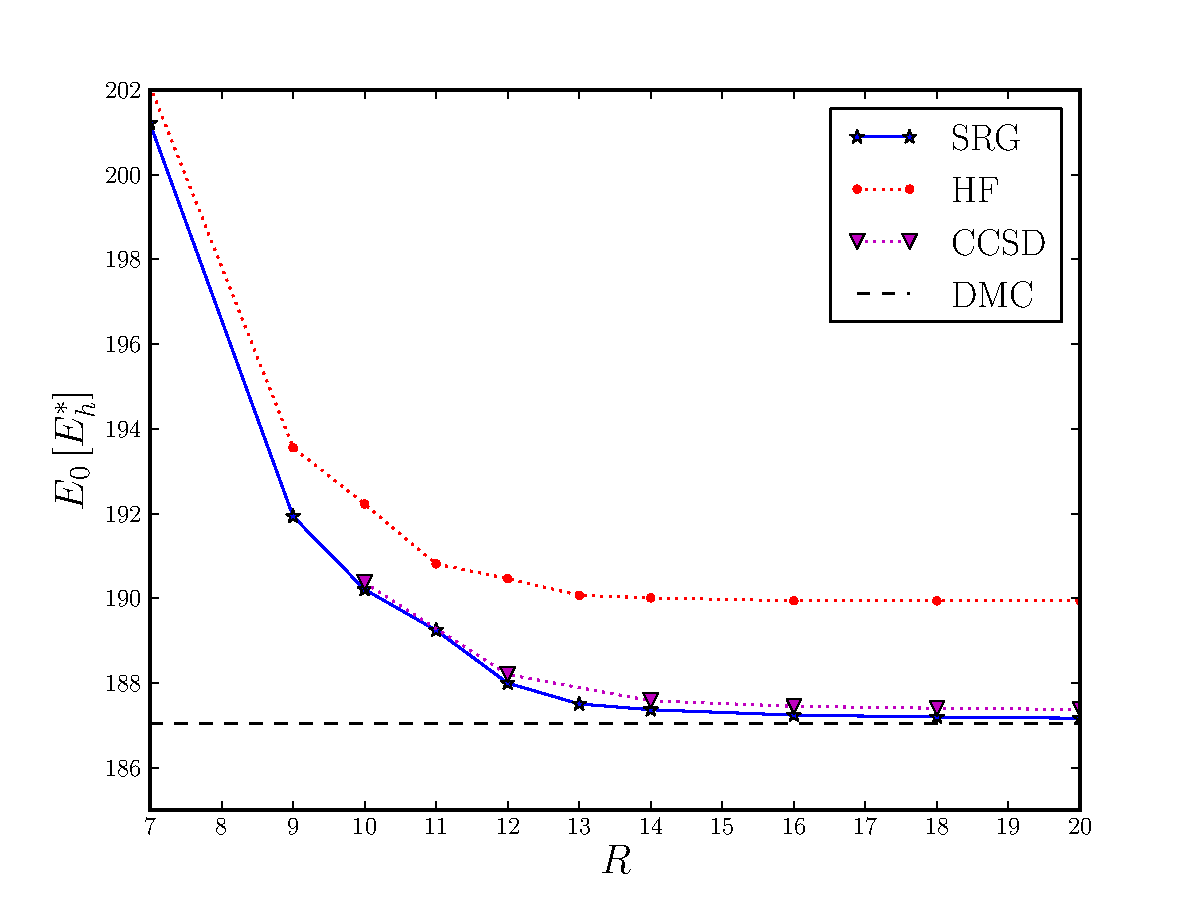
\includegraphics[width=0.38\textwidth]{figures/30parthw05.pdf}
        }\\ % ------- End of the first row ----------------------%
        \subfigure[Results for $N=30$ and $\omega=0.28$ ]{
            \label{fig:N30hw028}
            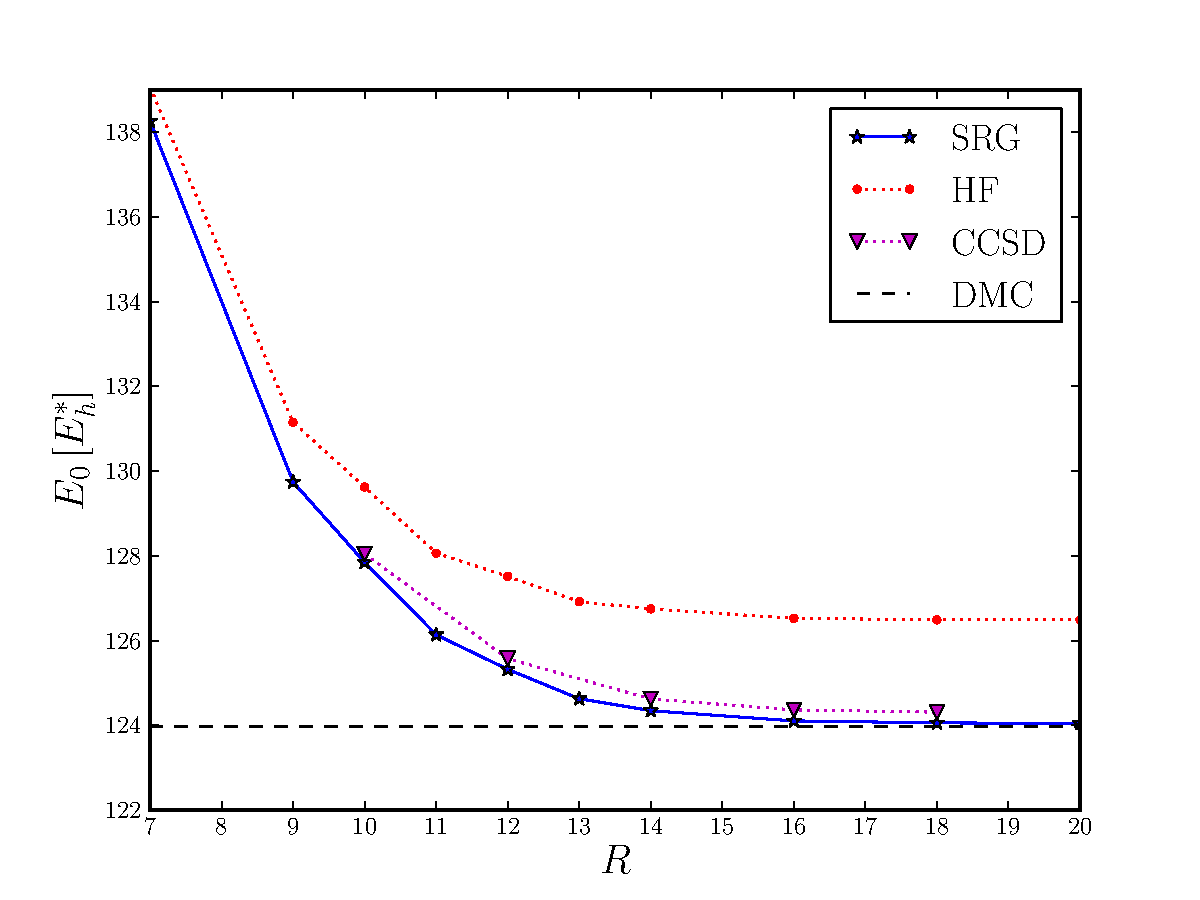
\includegraphics[width=0.38\textwidth]{figures/30parthw028.pdf}
        } \subfigure[Results for $N=30$ and $\omega=0.1$ ]{
            \label{fig:N30hw01}
            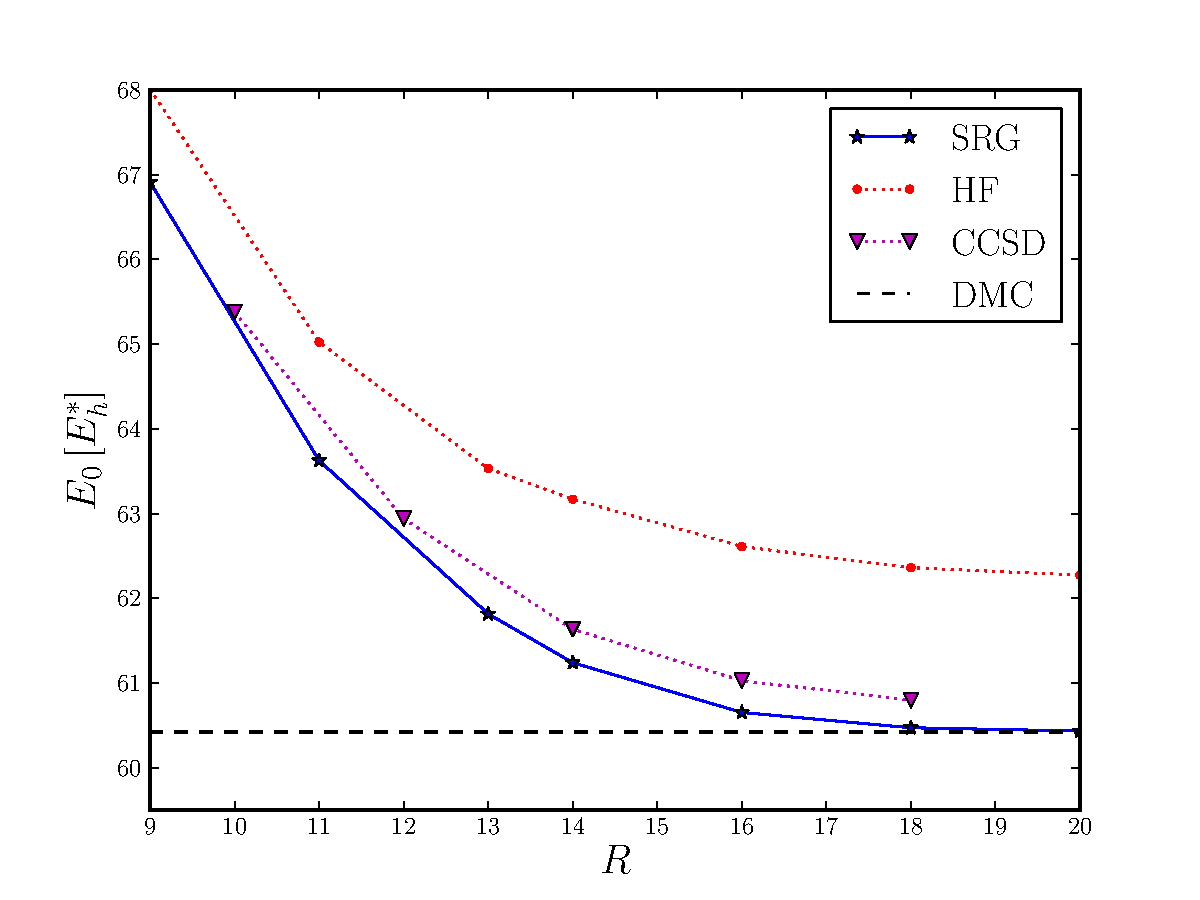
\includegraphics[width=0.38\textwidth]{figures/30parthw01.pdf}
        }
    \end{center}
    \caption{Comparison of our IM-SRG(2) ground state energies (SRG)
      for circular quantum dots for $N=30$ and different values of
      $\omega$. The results are compared with diffusion Monte
      Carlo (DMC), coupled cluster at the level of singles and doubles
      (CCSD), full configuration interaction (FCI) and Hartree-Fock
      calculations (HF) as functions of the number of major oscillator
      shells $R$. A harmonic oscilaltor basis has been used, with an
      unrenormalized Coulomb repulsion and White's generator. All
      energies in atomic units.}
   \label{fig:N30}
\end{figure}



\begin{figure}%[hbtp]
     \begin{center}
        \subfigure[Results for $N=42$ and $\omega=1.0$ ]{
            \label{fig:N42hw1}
            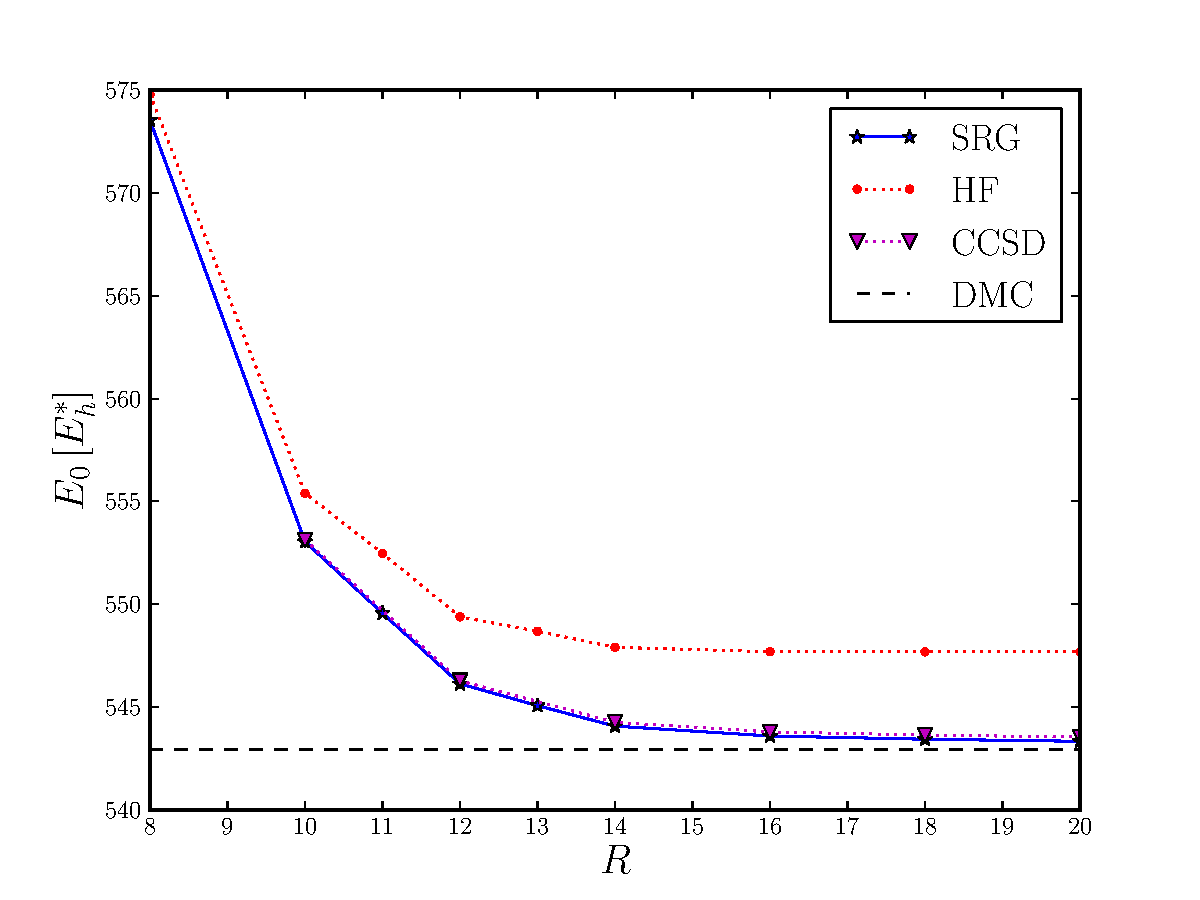
\includegraphics[width=0.38\textwidth]{figures/42parthw1.pdf}
        } \subfigure[Results for $N=42$ and $\omega=0.5$ ]{
           \label{fig:N42hw05}
           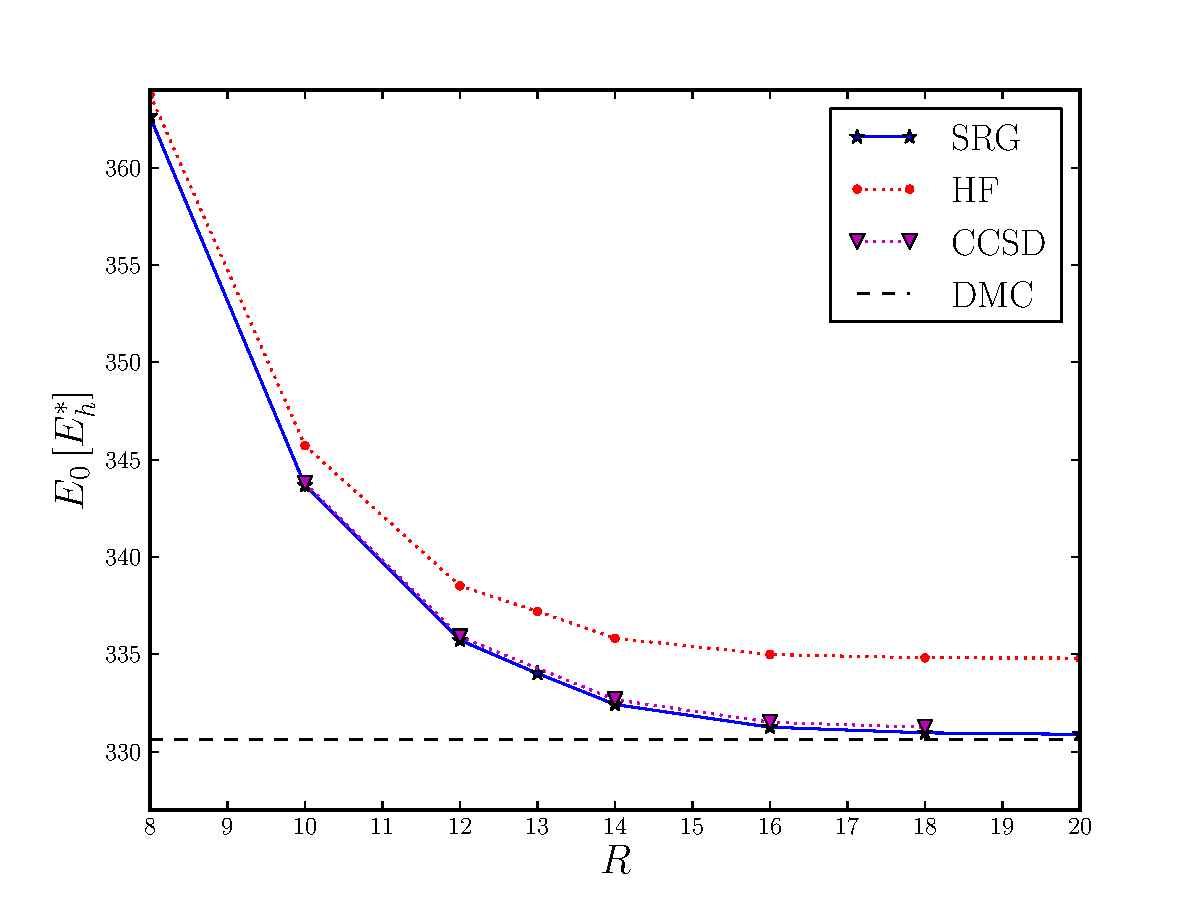
\includegraphics[width=0.38\textwidth]{figures/42parthw05.pdf}
        }\\ % ------- End of the first row ----------------------%
        \subfigure[Results for $N=42$ and $\omega=0.28$ ]{
            \label{fig:N42hw028}
            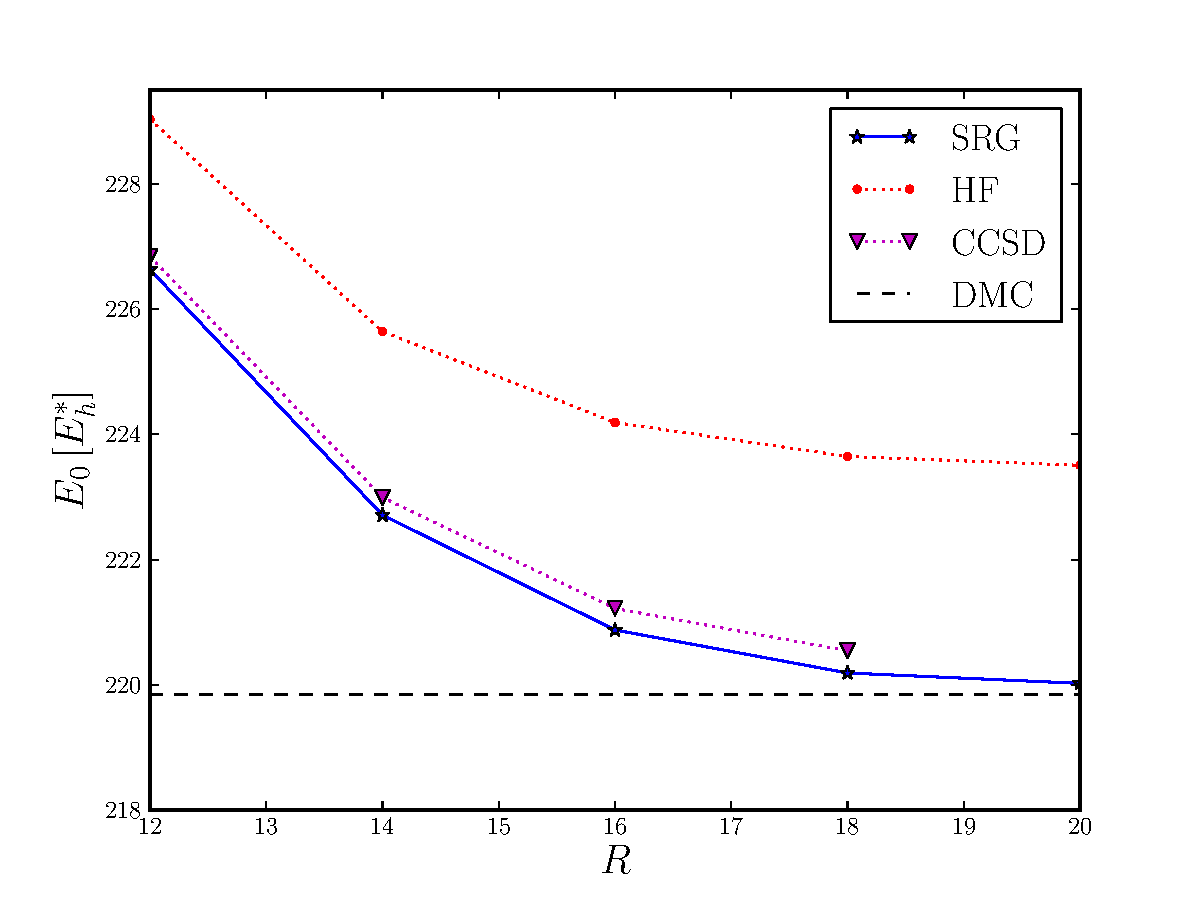
\includegraphics[width=0.38\textwidth]{figures/42parthw028.pdf}
        } \subfigure[Results for $N=42$ and $\omega=0.1$ ]{
            \label{fig:N42hw01}
            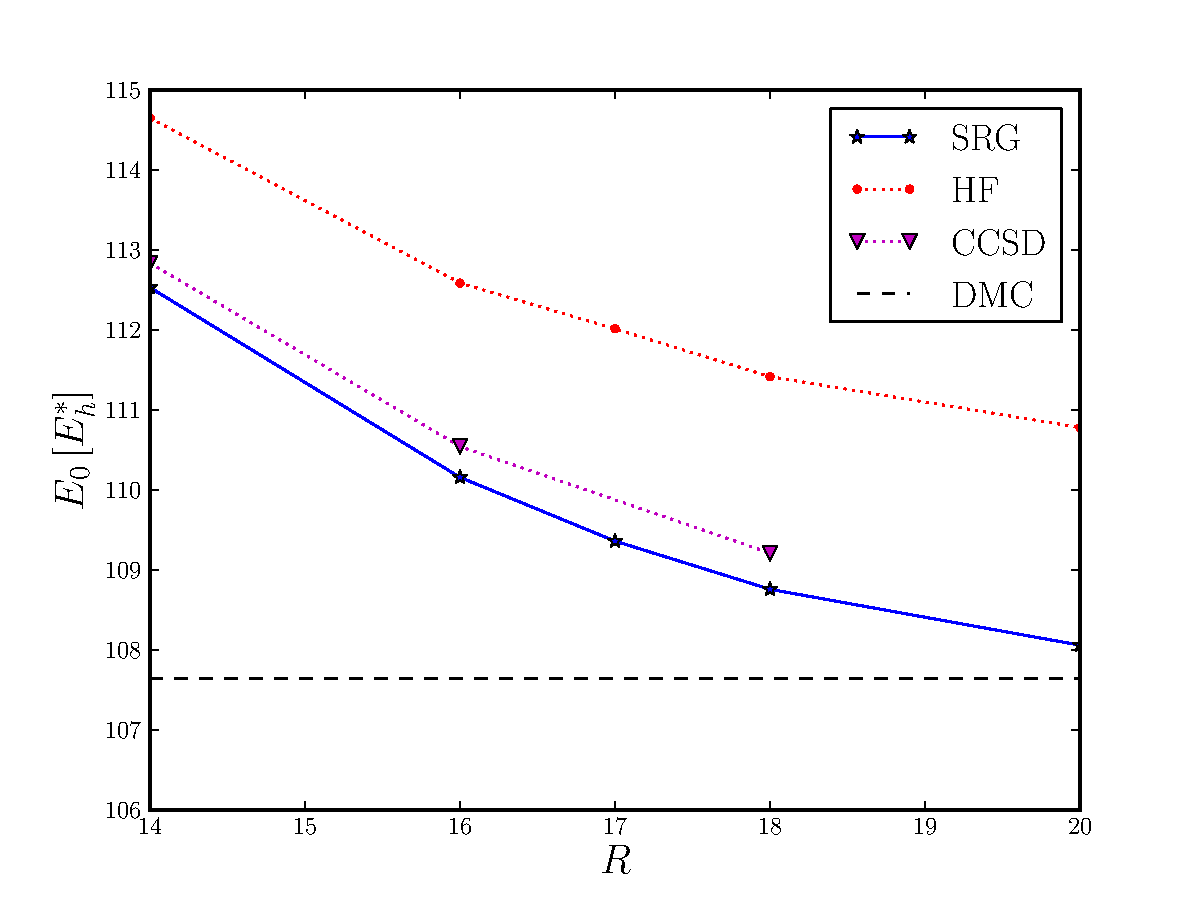
\includegraphics[width=0.38\textwidth]{figures/42parthw01.pdf}
        }
    \end{center}
    \caption{Comparison of our IM-SRG(2) ground state energies (SRG)
      for circular quantum dots for $N=42$ and different values of
      $\omega$. The results are compared with diffusion Monte
      Carlo (DMC), coupled cluster at the level of singles and doubles
      (CCSD), full configuration interaction (FCI) and Hartree-Fock
      calculations (HF) as functions of the number of major oscillator
      shells $R$. A harmonic oscilaltor basis has been used, with an
      unrenormalized Coulomb repulsion and White's generator. All
      energies in atomic units.}
   \label{fig:N42}
\end{figure}



\begin{table}
\begin{center}
\caption{Ground state energy (in atomic units) of a circular quantum
  dot, with $N$ particles and oscillator frequency $\omega$. The
  IM-SRG(2) results are given for $R=20$ shells (except for the $N=56$
  results which are for $R=18$), employing a Hartree-Fock basis, a
  bare Coulomb interaction and White's generator. For $N=42$ and
  $\omega=0.1$ results are presented up to $R=22$ major shells. The
  results labelled IM-SRG(2)$_{R\rightarrow \infty}$ are obtained
  using the extrapolation formula of Eq.().}
\label{tab:SRGDMC-R20}
\begin{tabular}{ccccc}
\hline\hline
$N$ & $\omega$ & IM-SRG(2) &IM-SRG(2)$_{R\rightarrow \infty}$ & DMC \\
\hline
6 & 1.0 & 20.1583 & 20.1468   & 20.1593(1) \\
& 0.5&11.7690  & 11.7631 &11.7848(1) \\
& 0.28& 7.5713 &   7.5695 &7.6002(1) \\
& 0.1& 3.4962  &  3.4977 &3.5539(1)\\
\hline
12&1.0 & 65.7280 & 65.6990  & 65.7001(1) \\
&0.5 &39.1631 &  39.1473 & 39.1596(1)\\
&  0.28&25.6212 &  25.6140& 25.6358(1)\\
&  0.1&12.2223 &  12.2234 & 12.2698(1)\\
\hline
20& 1.0&155.9737 & 155.9130  & 155.8822(1)\\
&  0.5&93.9219 &   93.8853 &93.8752(1)\\
&  0.28&61.94362 & 61.9240 &61.9268(1) \\
&  0.1&29.95263 &29.9565  & 29.9779(1)\\
\hline
30& 1.0& 308.7673 & 308.6053 & 308.5627(2) \\
 & 0.5& 187.1671& 186.8340 &187.0426(2)\\
 & 0.28&124.0410 & 123.7171 & 123.9683(2) \\
 & 0.1& 60.4319& 60.1158 & 60.4205(2)\\
\hline
42& 1.0&543.3398 & 543.3304 & 542.9428(8) \\
 & 0.5&330.8885 & 330.8425 & 330.6306(2)\\
 & 0.28&220.0226 & 219.9534y &219.8426(2) \\
 & 0.1& 107.7851&  106.8074& 107.6389(2)\\
 \hline
56& 1.0& 880.4159 &  & 879.3986(6) \\
 & 0.5& 538.8199 & & 537.353(2)\\
 & 0.28&360.83689  &  & 358.145(2) \\
\hline
\end{tabular}
\end{center}
\end{table}




In Figure \ref{fig:gs} we show the calculated ground state energies from
Hartree-Fock, second-order (M\o ller-Plesset) perturbation theory (MPPT), and
IMSRG.  The exact result from diffusion Monte Carlo (DMC) is also shown as a
dashed line in systems where it is known \cite{PhysRevB.84.115302}.

Both perturbation theory and IMSRG add corrections in addition to the
Hartree-Fock results to recover the correlation energy and they do quite well
in recovering the correlation energy in the system.  Compared with MPPT, IMSRG
generally converges faster, although does not always converge to the DMC
result.  Generally speaking, IMSRG is closer to the DMC result as the number
of particles increases.

There are a few cases where the IMSRG over-corrects the result, leading to a
ground state energy that is lower than the exact result.  This is not
unexpected given that, unlike Hartree-Fock, IMSRG is non-variational.  These
tend to occur when the number of particles is few, or the frequency is very
low (high correlation).  However, MPPT does not do much better in the high
frequency regimes as it often converges slower than IMSRG.

[[Q: should we discuss the absolute/relative correction plots?]]

For our addition and removal energy calculations, the results are summarized
in Figure \ref{fig:add} and Figure \ref{fig:rm} respectively.  The figures
show the the addition/removal energies for Hartree-Fock, combined with IM-SRG
and/or QDPT (Hartree-Fock is always included, as usual) [[better way to
explain this? the figure labels are somewhat misleading too]].  The DMC
results are also shown via dashed lines where they are known.

From these results, we see that the QDPT corrections add a substantial
contribution to the results of both Hartree-Fock with and without IM-SRG.
[[quantify ``substantial'' numerically]]

For the IM-SRG results, there is a small asymmetry between the behavior of our
removal and addition energies: we find that removal energies tend to be more
accurate and its behavior is relatively stable with respect to the number of
shells. [[why]]

Interestingly, the addition energy of Hartree-Fock with second-order QDPT
appears to surpass the accuracy of that of IM-SRG with second-order QDPT.
This is likely coincidental, as the third-order QDPT dramatically worsens the
result.

Both Hartree-Fock and IM-SRG results worsen as the frequency decreases, which
is not unexpected since the correlations become much more dominant.  The
Hartree-Fock appears to perform much worse, however, as the results converge
much more slowly as the number of shells increases.

We also note that IM-SRG with 2 particles and frequency 0.1 generally fail to
give any result as the ODE solver eventually leads to divergence [[Why?]]
This seems to be a particular quirk associated with this specific system and
does not usually occur in other systems except in a few extreme, isolated
cases where there are far too few unoccupied states.

\section{Conclusions}
\label{sec:conclusions}

We demonstrated the use various many-body theories, Hartree-Fock method, M\o
eller-Plesset perturbation theory, IM-SRG, as well as quasidegenerate
perturbation theory to calculate ground state as well as addition and removal
energies of two-dimensional quantum dots.  We showed that these methods, when
combined, can give a good approximate description of the systems at moderate
cost compared to near-exact but much more expensive methods such as FCI and
DMC.

For ground state energy, we showed that the convergence of IM-SRG is generally
faster than that of MPPT, and the results are typically closer to the exact
results.  Similarly, we found that IM-SRG improves the rate of convergence of
the addition and removal energies, both as the order of perturbation theory
increases and as the number of shells increases.

There are several directions in which the calculations may be improved.  One
can attempt to improve the IM-SRG approximation by incorporating some of the
missing higher-body terms in the commutator.  This would also provide some
insight into the rate of convergence with respect to the operator truncation.
While some of the higher-body terms can be rather costly to compute --
rendering a full 3-body IM-SRG quite expensive -- certain additional
approximations may be made to alleviate this without incurring the full cost
of evolving 3-body operators [[Ref?]].

[[As noted earlier [[haven't written that yet]], the application of IM-SRG
removes a large portion of the QDPT diagrams, which is beneficial as it
increases the efficiency of the QDPT calculations.  However, many of these
diagrams can also be eliminated further through an infinite resummation scheme
[[Any good refs for this?]], which would further reduce the number of diagrams
in QDPT, especially those of lower order, whic would likely increase the
accuracy of the result.]]

It would also be useful to investigate how the results obtained with finite
number of shells in the basis are related to those obtained with an infinite
number of shells in the basis.  [[Ref: paper on IR/UV extrapolation]] With a
good theoretical foundation, a model of how the observables converge with
respect to the size of the basis may be used to extrapolate the results to
infinite-basis limit.  This would also enable us to perform cheaper
calculations with fewer shells and optimistically extrapolate results for
large systems that would be otherwise infeasible to compute.

We note that this calculation was done entirely using the traditional approach
of using a high-order ODE solver to solve the flow equation.  A new technique
developed by T. Morris [[Ref?]] uses an alternative approach that obviates the
need for a high-order ODE solver, leading to much more efficient computations
and also allowing operators of other observables to be evolved with greater
ease.  Implementing this approach would be beneficial as it would allows us to
study the accuracy and convergence of other observables beyond energy and
energy differences.

Implementation-wise, our current code constructs the two-particle basis as
simple Slater determinants without any angular momentum coupling.  This
approach is often referred to as \textit{m-scheme} in nuclear physics.  This
method is simple and works well for general systems, but it does not fully
exploit the circular symmetry present in the quantum dot system.  A more
efficient approach is to use angular momentum coupling to generate the
two-particle basis, which is known as \textit{j-scheme} in nuclear physics.
Combined with the symmetries of the Hamiltonian, this can significantly reduce
the amount of computation required in this system, albeit at the cost of
increasing the complexity of the implementation.

A more technical issue is its lack of parallelization: currently, the code
makes very little use of parallelism and therefore does not scale well on
modern clusters.  As the problem is not embarrassingly parallel, implementing
parallelism does introduce additional complications that must be considered.
Distributing the workload across multiple nodes can significantly reduce the
cost of the calculations, allowing larger systems to be studied.

\begin{acknowledgments}
 This work was supported by the 
National Science Foundation Grant No.~PHY-1404159 
(Michigan State University) and by the Research
Council of Norway under contract ISP-Fysikk/216699. 
\end{acknowledgments}

\bibliography{paper}
\bibliographystyle{apsrev4-1}
\end{document}



\documentclass[aps,twocolumn,showpacs,floatfix,nofootinbib,preprintnumbers,superscriptaddress,amsmath,amssymb]{revtex4-1}

\usepackage{graphicx}
\usepackage{epsfig}
\usepackage{bm}
\usepackage{color}
\usepackage{float}
\usepackage{dcolumn}
\usepackage{subfigure}
\usepackage{multirow} 

\newcommand{\lb}{\left(}
\newcommand{\rb}{\right)}
\newcommand{\ad}{a^{\dagger}}
\newcommand{\Hd}{\hat{H}^{\rm d}}
\newcommand{\Ho}{\hat{H}^{\rm od}}
\newcommand{\be}{\begin{equation}}
\newcommand{\ee}{\end{equation}}
\newcommand{\T}{\hat{T}_{\rm rel}}
\newcommand{\da}{^\dagger}
\newcommand{\lla}{\left\langle}
\newcommand{\rra}{\right\rangle}
\newcommand{\llb}{\lbrace}
\newcommand{\rrb}{\rbrace}
\newcommand{\rv}{\mathbf{r}}

%Jorgen commands
\newcommand{\OP}[1]{{\hat{#1}}}
\newcommand{\ket}[1]{\left| #1 \right>}
\newcommand{\bra}[1]{\left< #1 \right|}
\newcommand{\braket}[2]{\left\langle #1 | #2\right\rangle}




\section{Results}
\label{sec:results}
In this section, we discuss the IM-SRG results for the ground-state
energies of closed-shell systems. In subsection \ref{subsec:Wegner},
we start with Wegner's canonical generator. Numerical instabilities in
the integration process, as well as a rather slow convergence as
function of the number of oscillator shells, motivate the use of a
Hartree-Fock basis and the Coulomb interaction. Since higher
correlations still lead to stiff equation systems, we change in
subsection \ref{subsec:White} to White's generator. In particular, we
give an overview of the IM-SRG(2) ground state energies for
closed-shell systems up to $N=42$ particles and compare with other
\textit{ab initio} many-body methods.\\ In all our calculations, we
perform the integration of the flow equations using the algorithm
developed by Shampine and Gordon \cite{shampine1975computer}. This
algorithm solves linear systems of differential equations based on the
implicit Adams method, which is a multi-step method of variable
order. Source code is freely available \cite{odesolver}.





\section{Conclusions}
\label{sec:conclusions}
We have used IM-SRG to study the ground state energy of circular,
two-dimensional quantum dots up to $N=42$ particles. We utilized two
different generators, Wegner's and White's one, and realized that
Wegner's generator results in stiff equation systems, whereas White's
generator has much better numerics and is computationally more
efficient. Moreover, we found out that the use of an Hartree-Fock
basis improves numerical stability enormously, whereas analogous to
previous FCI \cite{Kvaalcode} and CCSD \cite{PhysRevB.84.115302}
calculations, the use of an effective interaction improves convergence
of the ground state energy as function of the number of oscillator
shells.  Our IM-SRG(2) results are in excellent agreement with other
many-body methods, in particular DMC, which can be considered as more
or less exact benchmark. For more than six particles, we lie in all
cases closer to the DMC result than corresponding CCSD calculations
do.

Until now, we have applied the SRG flow equations in m-scheme only. A
next step, which we are currently working on, is to perform the
calculations in j-scheme. This allows for further simplifications of
the flow equations, such that numerical calculations get even more
efficient.  Moreover, one aspect of great interest is to extend
IM-SRG(2) to IM-SRG(3), where all operators are truncated one a
three-body instead of a two-body level. A comparison of both results
would give insight into the significance of higher correlations and it
would allow to analyse the convergence behaviour of the IM-SRG
hierarchy of truncation. However, since this is expected to be
computationally highly expensive, a first alternative would be not to
look at the whole IM-SRG(3) evolution, but to restrict oneself just to
certain additional terms, in order to get an impression of how
important excitations beyond the IM-SRG(2) level are. Since we use an
initial two-body Hamiltonian, one particular possibility is not to
save the induced three-body interactions explicitly, but to include
their loop terms in the calculations for lower-body interaction
terms. Work along these lines is in progress.\\ Furthermore, we plan
to apply these improvements not only to quantum dots, but to extend
our studies to nuclear and/or atomic systems, which opens up an even
larger range of applications.

%
\begin{acknowledgments}
  We thank Christoffer Hirth, Simen Kvaal and Veronica Olsen for
  several discussions. This work was supported by the Research Council
  of Norway under contract ISP-Fysikk/216699. This research used
  computational resources of the Notur project in Norway.
\end{acknowledgments}


\bibliography{srg}
\bibliographystyle{apsrev4-1}

\end{document}











The Hilbert spaces MR and PR is much closer in dimensionality than MR and PNP R . We
will therefore assume that we can use the same error formula for the spaces MR and PR .
As we will see later, this formula seems to hold very well for the systems we are studying.
We will also assume that ν(R) is negligible and rewrite Eq. (5.7) on the form
∞
∆E ≈ b ∑ (NP + r) r−c , b ∈ R.
(5.10)
r=R+1
This assumption is justified by Kvaal’s [16] results. He has performed FCI calculations on
two dimensional quantum dots in the energy cut basis with 3, 4 and 5 particles, and for these
systems ν(R) is shown to be small. Also, since PR ⊂ MR , we expect ν(R) to decay even
faster in the direct product basis.
5.3
Extrapolation Formulas
We have used Eq. (5.10) to parametrize the energy as a function of the number of shells.
R
E(R) ≈ a − b ∑ (NP + r)r− c ,
(5.11)
r=1
where a, b, c are real constants. This formula has an error ∼ E(R)ν(R), and consequently
it will become more accurate as R increases and ν(R) becomes small. This means that we
ˆ ˆˆ
should avoid extrapolations with energies ⟨PR H PR ⟩ for small R.
We also want to find the extrapolated energy at R → ∞ given that we know the optimal
values of a, b, c. We notice that E(∞) can be written in terms of the Riemann zeta function
ζ(c) such that
lim E(R) ≈ a − b[NP ζ(c) + ζ(c − 1)],
R→∞
where ζ(c) = ∑∞ r−c , which is known to converge for all c > 1.
r=1
34







In this section, we will calculate a set of extrapolated energies and compare these to
Diffusion Monte Carlo (DMC) energies which are not affected by a basis incompleteness
error. We use the extrapolation formula Eq. (5.11)
R
E(R) ≈ a − b ∑ (N + r)r−c ,
(25.1)
r=1
where N is the number of particles, R + 1 is the number of shells and a, b, c ∈ R are
constants. A curve fit of the FCIQMC values to E(R) yields the optimal parameters a, b, c.
The extrapolated energy is taken at the limit R → ∞, and the error is estimated using Eqs.
(13.18) and (13.22) assuming that Eq. (25.1) is exact.
As we discussed earlier, the extrapolation formula has an uncontrolled error ∝ ν(R)
where ν(R) is an unknown function. ν(R) is however assumed to fall off quickly as a
function of R. This is justified by the results of Kvaal [16] together with general consid-
erations about the form of the function. As we will see in this section, this assumption
seems to hold well for the systems that we have threated. To minimize ν(R) and reduce the
extrapolation error, we have only used energies calculated with R ≥ 5.






